\NeedsTeXFormat{LaTeX2e}
\documentclass[a4paper,12pt,
headsepline,           % Linie zw. Kopfzeile und Text
oneside,               % einseitig
acronym,               % Abkürzungsverzeichnis
pointlessnumbers,      % keine Punkte nach den letzten Ziffern in Überschriften
bibtotoc,              % LV im IV
%DIV=15,               % Satzspiegel auf 15er Raster, schmalere Ränder   
BCOR15mm               % Bindekorrektur
%,draft
]{scrbook}
\KOMAoptions{DIV=last} % Neuberechnung Satzspiegel nach Laden von Paket helvet

\pagestyle{headings}
\usepackage{blindtext}

%Schönere URLs
\usepackage[hyphens,spaces]{url}

%für schönere Tabellen
\usepackage{array}
\usepackage{booktabs}
\usepackage{eurosym}

% für Texte in englischer Sprache
\usepackage[english]{babel}
\usepackage[utf8]{inputenc}
\usepackage[T1]{fontenc}

%für Grafiken
\usepackage{graphicx} % Required for inserting images

%zum Aufzählen mit Buchstaben
\usepackage[shortlabels]{enumitem}

%Paket für Farben
\usepackage{color}

%Grafiken zeichnen
\usepackage{tikz}
\usetikzlibrary{shapes, positioning, decorations.pathreplacing, arrows.meta,positioning,calc}

%Grafiken zeichen als BPMN mit eigenem Package
%verworfen und lieber als SVG eingebunden
\usepackage{svg}


% Styles für Petri-Netz-Elemente

% fancy quotes
\definecolor{quotemark}{gray}{0.7}
\makeatletter
\def\fquote{%
    \@ifnextchar[{\fquote@i}{\fquote@i[]}%]
           }%
\def\fquote@i[#1]{%
    \def\tempa{#1}%
    \@ifnextchar[{\fquote@ii}{\fquote@ii[]}%]
                 }%
\def\fquote@ii[#1]{%
    \def\tempb{#1}%
    \@ifnextchar[{\fquote@iii}{\fquote@iii[]}%]
                      }%
\def\fquote@iii[#1]{%
    \def\tempc{#1}%
    \vspace{1em}%
    \noindent%
    \begin{list}{}{%
         \setlength{\leftmargin}{0.1\textwidth}%
         \setlength{\rightmargin}{0.1\textwidth}%
                  }%
         \item[]%
         \begin{picture}(0,0)%
         \put(-15,-5){\makebox(0,0){\scalebox{3}{\textcolor{quotemark}{``}}}}%
         \end{picture}%
         \begingroup\itshape}%
 %%%%********************************************************************
 \def\endfquote{%
 \endgroup\par%
 \makebox[0pt][l]{%
 \hspace{0.8\textwidth}%
 \begin{picture}(0,0)(0,0)%
 \put(15,15){\makebox(0,0){%
 \scalebox{3}{\color{quotemark}''}}}%
 \end{picture}}%
 \ifx\tempa\empty%
 \else%
    \ifx\tempc\empty%
       \hfill\rule{100pt}{0.5pt}\\\mbox{}\hfill\tempa,\ \emph{\tempb}%
   \else%
       \hfill\rule{100pt}{0.5pt}\\\mbox{}\hfill\tempa,\ \emph{\tempb},\ \tempc%
   \fi\fi\par%
   \vspace{0.5em}%
 \end{list}%
 }%
 \makeatother

%Hurenkinder und Schusterjungen
\clubpenalty=10000
\widowpenalty=10000

%Für Abkürzungsverzeichnis
\usepackage{acronym}

% Helvetica als Standard-Dokumentschrift
\usepackage[scaled]{helvet}
\renewcommand{\familydefault}{\sfdefault} 

\usepackage{graphicx}

%Mehrere Zeilen auskommentieren
\usepackage{verbatim}

% Literaturverzeichnis mit BibLaTeX
\usepackage[babel,german=quotes]{csquotes}
%\usepackage[backend=biber]{biblatex}
%\bibliography{bibliography}

% Alternative mit Paket-Option backend=biber und \addbibresource
 \usepackage[backend=biber]{biblatex}
 \addbibresource{bibliography.bib}

% Für Tabellen mit fester Gesamtbreite und variabler Spaltenbreite
\usepackage{tabularx} 

% Besondere Schriftauszeichnungen
\usepackage{url}              % \url{http://...} in Schreibmaschinenschrift
\usepackage{color}            % zum Setzen farbigen Textes

\usepackage{amssymb, amsmath} % Pakete für Mathe-Umgebungen und -Symbole

\usepackage{setspace}         % Paket für div. Abstände, z.B. ZA
%\onehalfspacing              % nur dann, wenn gefordert; ist sehr groß!!
\setlength{\parindent}{0pt}   % kein linker Einzug der ersten Absatzzeile
\setlength{\parskip}{1.4ex plus 0.35ex minus 0.3ex} % Absatzabstand, leicht variabel

% Tiefe, bis zu der Überschriften in das Inhaltsverzeichnis kommen
\setcounter{tocdepth}{3}      % ist Standard

% Beispiele für Quellcode
\usepackage{listings}
\lstset{language=Java,
  showstringspaces=false,
  frame=single,
  numbers=left,
  basicstyle=\ttfamily,
  numberstyle=\tiny}

% hier Namen etc. einsetzen
\newcommand{\fullname}{Moritz Wüst}
\newcommand{\email}{Moritz.Wuest@uni-ulm.de}
\newcommand{\titel}{Increasing Sales Performance through \\  Process Mining -  A Case Study  \\ of  Lead Management at Bosch }

%Driving Sales Performance through Event-Driven Process Mining: The Lead Conversion Process at Bosch
%Driving Sales Performance: \\ Event-Driven Analysis of the \\ Lead Conversion Process at Bosch
\newcommand{\jahr}{2025}
\newcommand{\matnr}{3074927}
\newcommand{\gutachterA}{Prof.\,Dr.\,Manfred Reichert}
\newcommand{\emailGutachter}{Manfred.Reichert@uni-ulm.de}
%\newcommand{\gutachterB}{Prof.\,Dr.\,Un Leserlich}
\newcommand{\betreuer}{Maximilian Möller}
\newcommand{\emailBetreuer}{Maximilian.Moeller@uni-ulm.de}

% hier die Fakultät auswählen
%\newcommand{\fakultaet}{---  Im Quellcode anpassen nicht vergessen! ---}
\newcommand{\fakultaet}{Engineering, \\ Computer Science \\ and Psychology}
%\newcommand{\fakultaet}{Mathematik und\\Wirtschafts-\\wissenschaften}
%\newcommand{\fakultaet}{Medizin}
%\newcommand{\fakultaet}{Naturwissenschaften}

% hier das Institut einsetzen
\newcommand{\institut}{Institute of Databases and Information Systems}

% Informationen, die LaTeX in die PDF-Datei schreibt
\pdfinfo{
  /Author (\fullname)
  /Title (\titel)
  /Producer     (pdfeTex 3.14159-1.30.6-2.2)
  /Keywords ()
}

\usepackage{hyperref}
\hypersetup{
pdftitle=\titel,
pdfauthor=\fullname,
pdfsubject={Diplomarbeit},
pdfproducer={pdfeTex 3.14159-1.30.6-2.2},
colorlinks=false,
pdfborder=0 0 0	% keine Box um die Links!
}

% Trennungsregeln
\hyphenation{Sil-ben-trenn-ung}

\begin{document}
\frontmatter


% Titelseite
\thispagestyle{empty}
\begin{addmargin*}[4mm]{-10mm}

\hfill
\includegraphics[height=1.8cm]{images/logo_uulm_sw.png}\\[1em]

{\footnotesize
%{\bfseries Universität Ulm} \textbar ~89069 Ulm \textbar ~Germany
\hspace*{115mm}\parbox[t]{35mm}{\bfseries Faculty of\\
\fakultaet\\
% TODO hier Institut anpassen
\mdseries \institut}\\[2cm]

\parbox{140mm}{\bfseries \LARGE \titel}\\[2.5em]
{\footnotesize Project Paper at Ulm University}\\[3em]

{\footnotesize \bfseries Submitted by:}\\
{\footnotesize \fullname\\ \email}\\ \matnr\\[2em]
{\footnotesize \bfseries Supervisor:}\\                     
{\footnotesize \gutachterA\\ 
{\footnotesize \emailGutachter}
%\gutachterB
}\\[2em]
{\footnotesize \bfseries Advisor:}\\ 
{\footnotesize \betreuer}\\
{\footnotesize \emailBetreuer} \\
\\\\
{\footnotesize \jahr}
}
\end{addmargin*}


% Impressum
\clearpage
\thispagestyle{empty}
{ \small
  \flushleft
  Version \today \\\vfill
  \copyright~\jahr~\fullname\\[0.5em]
% Wenn Sie Ihre Arbeit unter einer freien Lizenz bereitstellen möchten, können Sie die nächste Zeile in Ihren Code aufnehmen. Bitte beachten Sie, dass Sie hierfür an allen Inhalten, inklusive enthaltener Abbildungen, die notwendigen Rechte benötigen! Beim Veröffentlichungsexemplar Ihrer Dissertation achten Sie bitte darauf, dass der Lizenztext nicht den Angaben in den Metadaten der genutzten Publikationsplattform widerspricht. Nähere Information zu den Creative Commons Lizenzen erhalten Sie hier: https://creativecommons.org/licenses/
%This work is licensed under the Creative Commons Attribution 4.0 International (CC BY 4.0) License. To view a copy of this license, visit \href{https://creativecommons.org/licenses/by/4.0/}{https://creativecommons.org/licenses/by/4.0/} or send a letter to Creative Commons, 543 Howard Street, 5th Floor, San Francisco, California, 94105, USA. \\
  Typesetting: PDF-\LaTeXe
}

% ab hier Zeilenabstand etwas größer 

%
%           ENDE STYLE-DEFINITION
%
%


%
%
%           AB HIER DOKUMENTEN-INHALT
%
%
%

\frontmatter
\pagenumbering{Roman} % Groß-römisch

\setstretch{1.2}


%Inhaltsverzeichnis
\tableofcontents

%Abkürzungsverzeichnung

\chapter{List of Abbreviations}
%nur verwendete Akronyme werden letztlich im Dokument angezeigt

\begin{acronym}[AAAAAAAAAA]
\setlength{\itemsep}{-\parsep}

\acro{aida}[AIDA]{Awareness, Interest, Desire and Action}
\acro{asumdm}[ASUM-DM]{Analytics Solution Unified Method for Data Mining}
\acro{aws}[AWS]{Amazon Web Services}
\acro{bant}[BANT]{Budget, Authority, Need, Timing}
\acro{bdo}[BDO]{Bosch Digital Office}
\acro{bpmn}[BPMN]{Business Process Model and Notation}
\acro{champ}[CHAMP]{Challenges, Authority, Money, Prioritization}
\acro{erp}[ERP]{Enterprise Ressource Planning}
\acro{kpi}[KPI]{Key Performance Indicator}
\acro{llcm}[LLCM]{L* Life-Cycle Model}
\acro{lmt}[LMT]{Lead Management}
\acro{meddic}[MEDDIC]{Metrics, Economic Buyer, Decision Criteria, Decision Process, Identify Pain, Champion}
\acro{odbc}[ODBC]{Open Database Connectivity}
\acro{pam}[PAM]{Process Adherence Manager}
\acro{pais}[PAIS]{Process-Aware Information System}
\acro{pql}[PQL]{Process Query Language}
\acro{sql}[SQL]{Structured Query Language}
\acro{vuca}[VUCA]{Volatility, Uncertainty, Complexity and Ambiguity}




%\newacronym{lcm}{LCM}{Least Common Multiple}

\end{acronym}

%Tabellenverzeichnis
\cleardoublepage
\phantomsection
\addcontentsline{toc}{chapter}{List of Tables}
\listoftables

%Abbildungsverzeichnis 
\cleardoublepage
\phantomsection
\addcontentsline{toc}{chapter}{List of Figures}
\listoffigures

\mainmatter
\chapter{Introduction}

\begin{fquote}[Alex Rinke] [CEO and Founder of Celonis] [2023] Processes are the engine that make value repeatable in every business.
 \end{fquote}

This statement was made by Alex Rinke, one of the founders of \textbf{Celonis}, Germany’s most valuable tech start-up, currently valued at around 18 billion euros \cite{celonis2024cloud100}. Celonis offers a web-based Process Mining platform that provides companies with insights into their operations, helping them identify inefficiencies, bottlenecks, and hidden potentials.  

As expectations for Process Mining software continue to grow, many traditional manufacturing companies, such as Robert Bosch, still face challenges in managing the complexity of their existing processes that have evolved over time. These processes however, have direct consequences on the attractiveness of products, services and define the work of every employee \cite{dumas_laRosa_mendling_reijers_2018}. In today’s world made up of \ac{vuca}, innovative approaches to acquire and retain customers are essential. One modern approach of customer acquisition is \textbf{Lead Management}.  

This paper aims to establish a link between Process Mining and Lead Management \textendash{} a connection which has received little attention in the academic literature so far \cite{LeadmanagementDataMining2021}. 

\newpage

\section{Initial Situation}

The Bosch Home Comfort Group uses Lead Management since early 2018. Until the COVID-19 crisis and sudden material shortages, little attention was given towards an active Lead Management. This changed dramatically in 2023, as decreasing demand for heating and cooling required active customer- and lead acquisition. The lead volume increased, however the lead management itself remained unchanged from its original form, its processes and measures were never analyzed. In advance to this study, Marketing and Sales departments of Bosch Germany had multiple questions that could not be answered by traditional data analytics through e.g. PowerBI. 

\section{Research Objective}

Goal of this project paper is to discover insights on Lead Management with the help of Process Mining. Specifically, the study aims to explore how Process Mining techniques can provide transparency into the lead acquisition- and conversion processes, identify inefficiencies, and generate data-driven insights that support decision-makers in optimizing sales activities. 

By performing a case study at Bosch, this project paper tries to combine Process Mining and Lead Management and demonstrate the potential of process-based analytics.

This research seeks to answer the question:

\begin{center}
    \textit{"How can process mining be utilized to optimize lead management and enhance sales performance at Robert Bosch GmbH?"}
\end{center}

\newpage

\section{Methodology}
First of all, this project paper provides the user with a general overview of Process Mining in chapter two and Lead Management in chapter three. There, a framework called \ac{llcm} is introduced which serves as the methodological basis to analyze the case study. Chapter four deals with the problem statement at Robert Bosch GmbH and the challenge of adapting Process Mining to a Lead Management use case. Following the \ac{llcm}, the data is extracted from existing systems, process models are created and questions are formulated to address and optimize the current Lead Management at Bosch.
Insights and improvements to those questions are presented in chapter five, a final conclusion with a critical appraisal is drawn in chapter six.


\begin{comment}

]%
\blindtext

\subsection{Bilder und Abbildungen}

Auch in einer wissenschaftlichen Arbeit können Bilder und Abbildungen zur Veranschaulichung und zur Illustration sachlicher Inhalte integriert und einfügt werden. Für Fotografien und Bilder unterstützt PDF-\LaTeX{} direkt \verb|jpg| und \verb|png|. Ansonsten empfiehlt es sich, Vektorgrafiken zu verwenden und diese als \verb|pdf| zu speichern. Sollte ein Bild einmal von zu viel weißem Raum umgeben sein, kann man mit dem Werkzeug \verb|pdfcrop| das Bild automatisch zuschneiden.

\begin{figure}[ht]
\centering
\includegraphics[width=.4\textwidth]{images/Suffix_tree_ABAB_BABA}
\caption{\label{fig:bild1}Beschreibung/Beschriftung des Bilds}
\end{figure}

Mit Hilfe eines Labels \verb|\label{fig:bild1}| kann man sich dann im fortlaufenden Text mittels eines Querverweises auf diese Grafik beziehen: \verb|\ref{fig:bild1}|. An der Stelle des ref-Kommandos platziert LaTeX die Nummer der Abbildung: \glq siehe Abbildung \ref{fig:bild1}\grq.


\subsection{Tabellen}
\label{sec:tabellen}

Seite \pageref{tab:beispieltabelle}, Abschnitt \ref{sec:tabellen}, enthält Beispieltabelle \ref{tab:beispieltabelle}. In vielen \LaTeX{}-Büchern finden sich gute Anleitungen zum Erstellen von Tabellen. Komplexere Tabellen können sinnvollerweise in Excel oder einer anderen Tabellenkalulation vorgefertigt und mit einem Umwandlungsprogramm oder -werkzeug in LaTeX-Quellcode konvertiert werden.

\begin{table}[h]
\begin{center}
\begin{tabular}{|lll|}
    \hline
	A & B & C \\
	\hline
	x & x & x \\
	x & x & x \\
	\hline
\end{tabular}
\end{center}
\caption{Eine kleine Beispieltabelle}
\label{tab:beispieltabelle}
\end{table}


\subsection{Formeln}

Mathematische Formeln lassen sich in der Umgebung  \verb|math| erzeugen. Die Kurz- Schreibweise lautet \verb|\( a^2+b^2=c^2 \)|;  hierbei steht die Formel dann im laufenden Text: \( a^2+b^2=c^2 \). Die kürzeste Form ist mit zwei \verb|$| um die Formel, z.B.~so: Wasser ist H$_2$O. \verb|H$_2$O|

Mit der Schreibweise \verb|\[ y=x^2 \]| wird die Formel mittig in einer eigenen Zeile gesetzt, z.B.

\[y = x^2 \]

Formeln in der Umgebung \verb|equation| werden mittig in einer eigenen Zeile gesetzt und fortlaufend nummeriert:

\begin{equation}
x_{1,2} = \frac{-b\pm\sqrt{b^2-4ac}}{2a}
\label{mitternachtsformel}
\end{equation}
Wenn wir z.B.~über die beliebte Mitternachtsformel (Gleichung \ref{mitternachtsformel}) Details im umliegenden Text schreiben wollen, lässt sich diese wie ein Bild oder eine Tabelle referenzieren, sofern man ihr ein Label zugewiesen hat..


\subsection{Programmier-Code}

Mehrzeiliger Programmier- und Quellcode kann mit \verb|verbatim| in einer Umgebung gesetzt werden:


  Dieser Text steht in einer verbatim-Umgebung und wird daher
  in Schreibmaschinenschrift geschrieben.
  LaTeX-Kommandos, z.B. \includegraphics[width=.6\textwidth]{bild.jpg}
  werden nicht interpretiert, sondern "verbatim" ausgegeben.


Schöner und professioneller lässt sich Programmier-Code mit dem \verb|listings|-Paket, eingeben, formatieren und ausgeben. Dazu kann man in der Präambel die Sprache angeben, in der die Quellcodes geschrieben sind.

\begin{lstlisting}
public class Hello {
    public static void main(String[] args) {
        System.out.println("Hello World");
    }
}
\end{lstlisting}

Innerhalb einer Zeile gibt man Wörter am Besten als \verb|\verb##| an, dabei erwartet \LaTeX{} zweimal das gleiche Zeichen als Begrenzer. Im Beispiel ist dies die Raute \verb|#|, man kann aber auch jedes andere Zeichen nehmen, z.B. das Plus $+$.



\section{Text}

Textteile können bei Bedarf mit dem Befehl \verb|\emph{}| \emph{hervorgehoben} werden. Falls in einem Satz ein Punkt vorkommt, macht man danach kein Leerzeichen sondern eine Tilde (\verb|z.~B.~so!|), denn dann fügt \LaTeX{} den korrekten Abstand ein, z.~B.~so!


In der Präambel der vorliegenden tex-Datei gibt es den Befehl \verb|hypenation|, der zur Silbentrennung da ist. \LaTeX{} verfügt zwar über  eine eingebaute Silbentrennung, die jedoch bei manchen Wörtern falsch trennt. Damit diese Wörter korrekt getrennt werden, gibt man sie dann mit dem Befehl in der Präambel an\footnote{Das Wort \emph{Silbentrennung} ist hier das Beispiel}.

Fußnoten werden mit dem Befehl \verb|footnote| mitten in den fortlaufenden Text eingefügt. \footnote{Wie man schon im vorherigen Absatz sehen konnte.}

In wissenschaftlichen Arbeiten muss man des öfteren andere Arbeiten zitieren. Dazu nutzt man die Stiloptionen und Zitierbefehle des Pakets \verb+biblatex+, z.\,B.\,\verb|numeric| (=Standard-Stil) oder \verb|verbose| resp. \verb|\cite{name}| oder \verb|\autocite{name}|. In eckigen Klammern kann man noch die Seitenzahl angeben, falls notwendig. Der Name ist ein Schlüssel aus der Datei \verb|bibliography.bib|. Falls einmal ein Werk nur indirekt zu einem Teil der Arbeit beigetragen hat, kann man es auch mit \verb|nocite| angeben, dann landet es in der Literaturliste, ohne dass es im Text ausdrücklich zitert wird.


\subsection{Weiterführendes}

Zum Schluss sei auf die Vielzahl an Büchern zu \LaTeX{} verwiesen. In jeder Bibliothek wird sich eine Einführung finden, in der dann weitere Themen wie mathematische Formeln, Aufbau von Briefen und viele nützliche Erweiterungen besprochen werden.

\end{comment}
% hier weitere Kapitel einbinden

\usetikzlibrary{arrows.meta, positioning}


\chapter{Process Mining}

With the increasing complexity of modern day \ac{erp} systems, it has become a challenge to document all the business logic and processes that take place in such a system \cite{dumas_laRosa_mendling_reijers_2018}. Process Mining with its self-generating charts and documentations from existing datasets of such systems is a potential solution to this problem. Initial Research on Process Mining was performed by Jonathan E. Cook with his paper ``Automated Process Discovery through Event-Data Analysis'' in the year of 1996. Another important researcher on Process Mining is \textbf{\citeauthor{AalstSpaghetti}}, who worked with many other researchers on the ``Process Mining Manifesto'' in 2012. In this work, Process Mining is positioned as being closely related to Data Mining, which focuses on extracting insights from large datasets \cite{processminingmanifesto}.

To understand the relationship between information systems and Process Mining, three fundamental concepts are introduced: \textit{play-in}, \textit{play-out}, and \textit{replay} \cite{vanDerAalst2012ProcessMiningOverview}. \textit{Play-out} refers to the classical use of process models. After a process is executed, the execution log contains all traces from the prior execution. When a software system manages and executes processes involving people, applications, or information sources, it is called a  \ac{pais}. \ac{pais} therefore can be seen as \textit{play-out} engines, which create traces according to the model \cite{AalstSpaghetti, ReichertWeber2012}. \textit{Play-in} marks the  opposite, as it uses an event log to create a process model \cite{vanderAalst2016_processmining_in_action}.
\textit{Replay} on the other side uses both an event log and a process model. The event log is played ``on top'' in comparison to the process model to find deviations and mismatches. Use Cases of replaying the model might be conformance checking, building predictive models and operational support (e.g. alerting) \cite{ReichertWeber2012}. 

Process Mining is based on on the general idea of Petri Nets \cite{Weske2024}. They are an important basis for process languages. They consist of places (can be seen as preconditions or states), transitions (actions or activities), and directed edges connecting places and transitions. An example can be seen in figure \ref{fig:petrinet}. 

The dynamic behavior of Petri Nets is represented by tokens and markings that run through the net while executing. Places can store one or multiple tokens, depending on the Petri Net type.  A transition fires if it is enabled \cite{ReichertWeber2012}. These Petri Nets now allow working with the execution log of e.g. a \ac{pais}. As Process Mining first started with Process Discovery, today it is combined with  Machine Learning to address inefficiencies and deviations \cite{reinkemeyer:2020}. 
In comparison to the \textit{data-centric} Data Mining, Process Mining  is \textit{process-centric} and focuses on \textit{fact-based} and \textit{truly-intelligence} analysis \cite{ReichertWeber2012}.


\begin{figure}%[h]
\centering
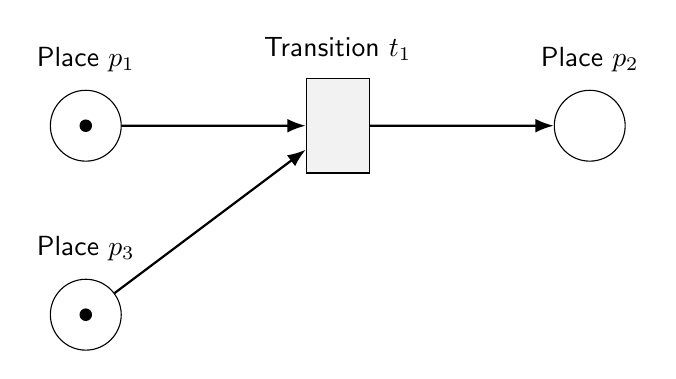
\begin{tikzpicture}[node distance=22mm, scale=0.8]

\tikzset{
  place/.style={circle, draw, minimum size=9mm, inner sep=0pt},
  transition/.style={rectangle, draw, minimum height=12mm, minimum width=8mm, fill=gray!10},
  token/.style={circle, fill=black, inner sep=1.6pt},
  >={Latex}
}

% Rest unverändert
% --- Titel / Kontext ---


% --- Netz-Knoten (mit absoluten Koordinaten) ---
\node[place] (p1) at (-8,1.5) {}; 
\node[transition] (t1) at (-4,1.5){}; 
\node[place] (p2) at (0,1.5) {}; 
\node[place] (p3) at (-8,-1.5) {}; 



%\node[place]      (p1) at (-10,-1.5)  {};   % erster Place links oben
%\node[transition] (t1) at (2.2,-1.5) {};  % erste Transition rechts davon
%\node[place]      (p2) at (4.4,-1.5) {};  % zweiter Place
%\node[transition] (t2) at (6.6,-1.5) {};  % zweite Transition
%\node[place]      (p3) at (8.8,-1.5) {};  % dritter Place



% --- Kanten ---
\draw[->, thick] (p1) -- (t1);
\draw[->, thick] (t1) -- (p2);
\draw[->, thick] (p3) -- (t1);


% --- Token als Markierung ---
\node[token] at (p1) {};
\node[token] at (p3) {};


% --- Beschriftungen ---
\node[above=1mm of p1] {Place $p_1$};
\node[above=1mm of t1] {Transition $t_1$};
\node[above=1mm of p2] {Place $p_2$};
\node[above=1mm of p3] {Place $p_3$};



\end{tikzpicture}

\caption{Petri Net Example with three Places and a Transition}
\label{fig:petrinet}
\end{figure}


%
%
\section{Event Log}

As already mentioned, the execution of one or several processes can be logged. This most essential part of process mining is the so-called \textbf{event log}. The execution log can be used for multiple purposes, such as monitoring, ensuring traceability, analysis as well as diagnosis \cite{ReichertWeber2012, Weske2024}. 
A minimum event log typically exists of three different columns, namely \textit{Case ID}, \textit{Activity} and \textit{Timestamp}. \textit{A User ID} is also beneficial and often mentioned, an example can be seen in table \ref{tab:minimal_event_log} \cite{ReichertWeber2012, reinkemeyer:2020}.   \\

\begin{table}[h]
\centering
\begin{tabular}{l | l | l| l}
\textbf{Case ID} & \textbf{Activity} & \textbf{Timestamp} & \textbf{User ID} \\
\hline
C01 & Approve Request & 2024-05-03 09:15 & U123 \\
\hline
C01 & Send Notification & 2024-05-03 09:18 & U088 \\
\hline
C02 & Validate Data & 2024-05-04 14:02 & U123 \\
\end{tabular}
\caption{Example of a minimal event log \cite{ReichertWeber2012}}
\label{tab:minimal_event_log}
\end{table}
\label{sec:lasagneshaphetti}

\newpage

Multiple instances of a Case ID are called a \textit{trace}, meaning a sequential flow of activities ordered by timestamp. 
In general, processes can be distinguished into two separated groups based on their complexity \cite{vanDerAalst2012ProcessMiningOverview}. One group, containing very complex and hard to follow process charts, is called \textit{spaghetti process}. The complexity reflexes the reality shown in the log files, hence it is not caused by the discovery algorithm, and the model is too complex to understand \cite{AalstSpaghetti}. The second category is called \textit{lasagna process} and describes the very opposite: highly structured, easy to understand, and displayable processes \cite{vanDerAalst2012ProcessMiningOverview}. 


\begin{figure}%[h]
\centering
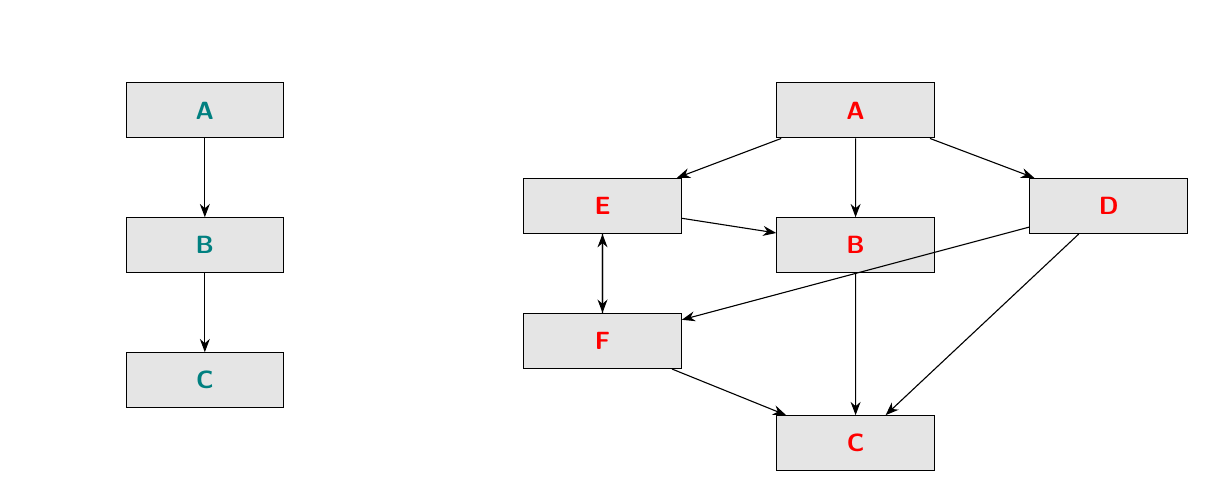
\begin{tikzpicture}[scale=0.7,
    every node/.style={draw, fill=gray!20, minimum width=2cm, minimum height=0.7cm, font=\small},
    >=Stealth]

% Linkes Diagramm
\node[draw=none, fill=none, minimum size=4.5cm, thick, teal, circle] (C1) {};
\node (A1) at (C1.center) [yshift=1.2cm] {\textcolor{teal}{\textbf{A}}};
\node (M1) [below=of A1] {\textcolor{teal}{\textbf{B}}};
\node (B1) [below=of M1] {\textcolor{teal}{\textbf{C}}};

\draw[->] (A1) -- (M1);
\draw[->] (M1) -- (B1);

% Untertitel (a)
%\node[draw=none, fill=none, below=0.4cm of B1, font=\small] {(a) Linear};

% Rechtes Diagramm
\node[draw=none, fill=none, minimum size=4.5cm, thick, red, circle, right=6cm of C1.center] (C2) {};
\node (A2) at (C2.center) [yshift=1.2cm] {\textcolor{red}{\textbf{A}}};
\node (N1) [below=of A2] {\textcolor{red}{\textbf{B}}};
\node (N2) [below right=0.5cm and 1.2cm of A2] {\textcolor{red}{\textbf{D}}};
\node (N3) [below left=0.5cm and 1.2cm of A2] {\textcolor{red}{\textbf{E}}};
\node (N4) [below=of N3] {\textcolor{red}{\textbf{F}}};
\node (B2) [below=of N1, yshift=-0.8cm] {\textcolor{red}{\textbf{C}}};

% Pfeile
\draw[->] (A2) -- (N1);
\draw[->] (A2) -- (N2);
\draw[->] (A2) -- (N3);
\draw[->] (N1) -- (B2);
\draw[->] (N3) -- (N4);
\draw[->] (N4) -- (B2);
\draw[->] (N2) -- (B2);
\draw[->] (N2) -- (N4);
\draw[->] (N3) -- (N1);
\draw[->] (N4) -- (N3);

% Untertitel (b)
%\node[draw=none, fill=none, below=0.4cm of B2, font=\small] {(b) Vernetzt};

\end{tikzpicture}
\caption{Expected Process vs. Process in Reality \cite{vanDerAalst2012ProcessMiningOverview}}
\label{fig_expectedprocess_vs_reality}
\end{figure}

By design, processes are supposed to follow a strict set of events (see process on the left in figure \ref{fig_expectedprocess_vs_reality}), however they often turn out to be more complex (see figure \ref{fig_expectedprocess_vs_reality} on the right) \cite{reinkemeyer:2020}. Reasons to this can be diverse, e.g. manual input, exception handling or errors inside the workflow engine \cite{vanDerAalst2012ProcessMiningOverview}. 

\newpage

\section{Quality Criteria}
There are in total six different quality criteria that can be assigned to process models to rate either the \textbf{quality of the event log} or the \textbf{quality of the process model} \cite{ReichertWeber2012}.

\subsection{Event Log}
Regarding quality of the event log, to \citeauthor{AalstSpaghetti} the selected log must contain a 
\begin{quote}
\textit{``representative sample of the model behavior.''} \cite{vanderAalst2016_processmining_in_action}
\end{quote}
Otherwise, conclusions of the process model cannot be made based on the event log since it is lacking information. \citeauthor{vanderAalst2016_processmining_in_action} mentions two different quality criteria for event logs: 

\textbf{Noise} describes a phenomenon where the event log contains traces that never or only very rarely happen in the real world. This does not refer to incorrect logging, more so there might be human input, interruption, or error handling. The evolving term of the $80/20$ model describes an ideal situation where $80\%$ of the behavior of the process model can be described by only $20\%$ of the variability of the event log. The remaining $80\%$    of the variability only makes up $20\%$ of the behavior and therefore can be seen as negligible \cite{vanderAalst2016_processmining_in_action}.

\textbf{Incompleteness} describes a phenomenon where the event log contains too few traces to create a process model that reflects reality. As real-world process models typically allow for thousands 
of different traces, it is unrealistic to assume that every possible trace is part of the event log \cite{vanderAalst2016_processmining_in_action, ReichertWeber2012}.

\newpage
\label{sec:quality_criteria}
\subsection{Process Modeling}
In process modeling, four fundamental and mutually competing quality criteria are typically considered: \textit{fitness}, \textit{simplicity}, \textit{precision}, and \textit{generalization} \cite{vanderAalst2011ProcessMining}. These criteria capture different aspects of model quality and are often in tension with one another, such that improvements in one dimension may lead to trade-offs in others. The construction of high-quality process models therefore requires a balanced consideration of all four criteria \cite{reinkemeyer:2020}. As shown in Figure \ref{fig:four_quality_dimensions}, \textit{fitness} measures how well a model can replay the observed event log, while \textit{precision} indicates how strictly the model restricts behavior to what is actually observed. In contrast, \textit{generalization} reflects the ability to allow plausible but unseen behavior, and \textit{simplicity} follows the principle of Occam’s razor by favoring models that are easy to understand. High-quality process models aim to balance these four criteria rather than optimizing any single one in isolation \cite{vanderAalst2011ProcessMining, Buijs2014DiscoveringNavigating}. 

\begin{figure}
    \centering
 
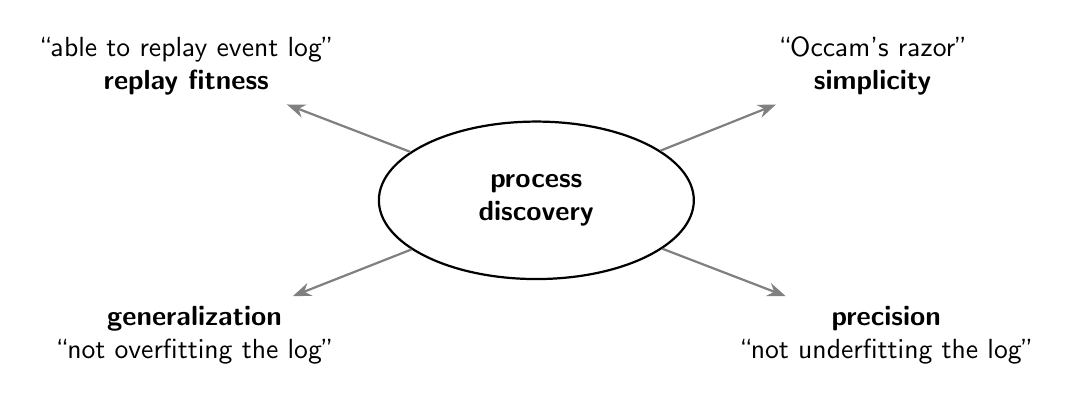
\begin{tikzpicture}[
    >=Stealth,
    every node/.style={align=center},
    arrow/.style={->, thick, gray}
]

% Zentrales Oval
\node[draw, ellipse, thick, minimum width=4cm, minimum height=2cm] (pd) {
    \textbf{process}\\
    \textbf{discovery}
};

% Oben links: replay fitness
\node[above left=0.5cm and 1cm of pd] (fitness) {
    ``able to replay event log''\\
    \textbf{replay fitness}
};
\draw[arrow] (pd) -- (fitness);

% Oben rechts: simplicity
\node[above right=0.5cm and 1.5cm of pd] (simplicity) {
    ``Occam's razor''\\
    \textbf{simplicity}
};
\draw[arrow] (pd) -- (simplicity);

% Unten links: generalization
\node[below left=0.5cm and 1cm of pd] (generalization) {
    \textbf{generalization}\\
    ``not overfitting the log''
};
\draw[arrow] (pd) -- (generalization);

% Unten rechts: precision
\node[below right=0.5cm and 1cm of pd] (precision) {
    \textbf{precision}\\
    ``not underfitting the log''
};
\draw[arrow] (pd) -- (precision);

\end{tikzpicture}
    \caption{Four Quality Dimensions of Process Discovery \cite{vanderAalst2011ProcessMining}}
    \label{fig:four_quality_dimensions}
\end{figure}


\section{Kinds of Process Ming}

In general, process mining is commonly divided into \textbf{process discovery}, \textbf{conformance checking}, and \textbf{process enhancement} \cite{vanderAalst2011ProcessMining, ReichertWeber2012, reinkemeyer:2020}. These three categories address different stages of the process lifecycle, ranging from the automated construction of process models from event data to the analysis and improvement of existing processes.


\subsection{Discovery}

Marking the original cause of Process Mining, Process Discovery  aims to automatically construct process models from event data without any prior knowledge of the underlying process structure. The goal is to derive a formal representation, such as a Petri net or \ac{bpmn} diagram, that captures the behavior recorded in the event log as accurately as possible \cite{dumas_laRosa_mendling_reijers_2018}.
Unlike traditional process modeling, which depends on interviews, documentation, and manual analysis, Process Discovery relies on empirical event data that reflect how processes are executed in reality \cite{vanderAalst2011ProcessMining}.

For example, \citeauthor{dumas_laRosa_mendling_reijers_2018} define general process discovery as 
\begin{quote}
    

\textit{``the act of gathering information about an existing process and organizing it.''} \cite{dumas_laRosa_mendling_reijers_2018} 

\end{quote}
and mention evidence-, interview- and workshop-based discovery. All three presume that involved people are familiar with the process. To overcome this dependency on subjective human input, Process Mining enables an automated form of process discovery based on execution logs. It can be used if the execution log is already present which is mined afterwards, no matter by hand or by an algorithm \cite{dumas_laRosa_mendling_reijers_2018, ReichertWeber2012}. This makes it a data-driven approach capable of uncovering deviations, hidden workflows, or bottlenecks that may not be apparent in the designed process models \cite{Bernard2016SalesProcessMining}. Problems come along when the process changes over time which may result in incorrect process models build by the discovery algorithm. To address this issue, there are techniques that try to identify different versions of the process \cite{ReichertWeber2012}.

\newpage 
Process Discovery techniques can be broadly divided into bottom-up and top-down approaches \cite{vanderAalst2022ProcessMiningHandbook}:
\begin{enumerate}
    \item \textbf{Bottom-up discovery} approaches start from the local relations between activities in the event log and build up the model incrementally. One of the most influential methods in this category is the $\alpha$-algorithm, introduced by van der Aalst and Weijters, which identifies relationships between activities based on their ordering in traces \cite{vanderAalst2011ProcessMining, vanderAalst2016_processmining_in_action}. However, it is vulnerable to noise \cite{OrtmeierFrameworkIntoLifeCycleAssessment}. 
    \item \textbf{Top-down discovery} approaches construct process models from a global perspective by continuously breaking down the event log into smaller versions. Inductive mining algorithms are a prominent example of this category \cite{OrtmeierFrameworkIntoLifeCycleAssessment}. Because they are more resilient to noise, they ensure the discovery of sound, block-structured models, which makes them suitable for more complex real-world applications \cite{vanderAalst2022ProcessMiningHandbook}.
\end{enumerate}

In business context, Process Discovery can be used on processes itself, on organizations perspectives, on social networks or staff aissignment rules \cite{ReichertWeber2012}.
A key aspect of modern Process Discovery is the trade-off between the already mentioned quality criteria in chapter \ref{sec:quality_criteria} \cite{AalstSpaghetti}. 

\subsection{Conformance}
Conformance checking deals with the analysis how far an execution log matches a given process model. Specifically, it can highlight discrepancies and therefore show problems that come along after real executions \cite{vanderAalst2022ProcessMiningHandbook, ReichertWeber2012}. It is relevant for business alignment and auditing. Conformance checking allows to create \ac{kpi}s such as \textit{"$85\%$ of the cases in this event log can be replayed by the model"} (compare \cite{ReichertWeber2012}). How the missing $15\%$ can be interpreted, depends on the use case. 

\citeauthor{AalstSpaghetti} introduces the two terms \textit{descriptive} and \textit{normative}. If the model can be seen descriptive, it needs to be changed to reach the maximum, e.g. $100\%$ re-playability. If the model can be seen normative, one has to distinguish between \textit{undesirable deviations} and \textit{desirable deviations}. These two angles always need to be considered before taking actions to change the process model \cite{ReichertWeber2012}.



\subsection{Enhancement}
Enhancement uses extension algorithms to improve an existing process model based on information from the execution log. Enhancements can be, for example, better decisions based on past execution inside \ac{pais} such as removal of bottlenecks or unplanned behavior \cite{vanderAalst2022ProcessMiningHandbook, ReichertWeber2012}. \citeauthor{vanDerAalst2012ProcessMiningOverview} mentions that information from the event log can be extracted to identify roles of people, e.g. those who frequently perform tasks. Enhancement also allows to add data mining technics, such as decision trees to explain behavior or build social networks from work flows \cite{vanDerAalst2012ProcessMiningOverview, ReichertWeber2012}.

\clearpage
\section{L$^{\ast}$ Life-Cycle Model}

\begin{figure}
    \centering
    \includegraphics[width=1.09\linewidth]{images/L_lifecycle.png}
    \caption{The L$^{\ast}$ Life-Cycle Model \cite{AalstSpaghetti, Esiefarienrhe2021}}
    \label{fig:placeholder}
\end{figure}


The L$^{\ast}$ Life-Cycle Model is a framework designed to streamline process mining application on both spaghetti as well as lasagne processes which have already been introduced in section \ref{sec:lasagneshaphetti}\cite{Esiefarienrhe2021}. It was initially created by \citeauthor{AalstSpaghetti} in 2012. As spaghetti processes require a lot of manual work to structure and extract valuable information, a framework was needed to structure the optimal process mining project management \cite{AalstSpaghetti}. As multiple frameworks exist for the adoption of process mining into various fields such as lifecycle assessment (cf. \cite{OrtmeierFrameworkIntoLifeCycleAssessment}), a dedicated framework for lead management is yet to be introduced. 

The L$^{\ast}$ Life-Cycle Model is already adopted to business fields of flexible processes (e.g. the healthcare sector in \cite{Esiefarienrhe2021}) and therefore suitable for less structured processes \cite{OrtmeierFrameworkIntoLifeCycleAssessment}.

The framework is divided into five different stages, where most of them run sequentially. Nevertheless, the interpretation of results after the creation of control-flow and process models allows returning to earlier stages, thereby supporting an iterative approach.

Stage 0, called \textbf{plan and justify}, is supposed to build the foundation and motivation for the process mining project. Resources need to be allocated, project milestones defined and a team needs to be built up. Projects can be distinguished between three different types:

\begin{enumerate}
    \item The \textit{data-driven project} start without a concrete question in mind. Managers, stakeholders, and business analysts hope to find meaningful insights after analyzing the event log of the process. The project therefore has an explorative character \cite{Esiefarienrhe2021}. 
    \item A \textit{question-driven project} starts with initial questions and aims to answer these questions during analyzing the data. Beneficial is the fact that the analyst always has a goal in mind and is not distracted by the sheer amount of capabilities by modern-day process mining software \cite{AalstSpaghetti, Esiefarienrhe2021}. 
    \item A \textit{goal-driven project} sets \ac{kpi} and aims to improve these e.g. via cost reduction or improved throughput times \cite{Esiefarienrhe2021}. 
\end{enumerate}

\citeauthor{AalstSpaghetti} recommends companies without much process mining experience to start with \textit{question-driven} since it helps to streamline resources \cite{AalstSpaghetti}.

Stage 1, called \textbf{Extract}, deals with extracting event logs, objectives and questions from affected systems. This step may the be most time-consuming task. Van der Aalst names the example of SAP Systems, where relevant data is stored in thousands of tables and finding the correct data can be very challenging. If the company has some existing process models, they can be used to exploit existing knowledge. Inside stage 1, the objectives of a goal-driven process mining projects have to be defined, as well as the questions of a question-driven project.

Stage 2, called \textbf{Create Control-Flow Model and Connect Event Log} deals with creating the real-world control-flow via discovery algorithms such as $\alpha$ -algorithm, heurisitic miner or fuzzy miner. This discovered model can be evaluated by conformance checking against traces. Challenges during discovery can be overfitting, underfitting and representational bias of the selected algorithm. However more complex algorithms such as the heuristic miner can deal with these problems quite well \cite{Bernard2016SalesProcessMining}. Subsequent analysis should only be done if the model reaches a good fitness, meaning the discovered model can replay most of the traces. Van der Aalst recommends a fitness above 0.8, anything below is considered low \cite{AalstSpaghetti}. However this only applies to spaghetti processes, since lasagna processes can be fully modeled anyways. The results of stage 2 can be used to answer first questions of a question-driven project \cite{Esiefarienrhe2021}.

Stage 3, called \textbf{Create Integrated Process Model}, aims to add additional perspectives to the control flow model. One perspective can be organizational, meaning department and user-specific data. This organizational data can be used to e.g. identify bottlenecks via long throughput times. These insights can be used to make adjustments within the organization to address the bottleneck \cite{Esiefarienrhe2021}.

Stage 4, \textbf{Operational Support}, deals with detection, prediction and recommendation of the process. Running data is required to make predictions and recommend actions. One action can be automated alerting based on specific paths that were followed by that process. Predictions can be sent to the persons working on the case to boost handling time. Stage 4 of the L* Life-Cycle model is the most ambitious stage and requires advanced IT infrastructure and live data connection to the source system. It is also only possible for lasagna processes, since spaghetti processes cannot be designed to follow predictable paths \cite{AalstSpaghetti, Esiefarienrhe2021}.



\chapter{Lead Management}

Lead Management is one part of the customer acquisition process. This process follows several phases, which is referred by multiple authors as the \textbf{Sales Funnel} or \textbf{Conversion Funnel}. 
While comparing different literature, it soon becomes clear that there is no exact definition of ``Lead Management'' \cite{Vossebein2024LeadManagement, WengerLeadmanagement2021}.

In 2024, \citeauthor{Vossebein2024LeadManagement} define a lead as 

\begin{quote}
\textit{``a potential new customer who expresses interest in a company's product or service by voluntarily providing their contact information. This may refer to either an individual or a company.''} \cite{Vossebein2024LeadManagement}
\end{quote} 

Lead Management describes the processes involved while generating, qualifying and conversion of leads into real sales. It cannot be bound to a specific department, however mostly sales and marketing areas are involved during Lead Management \cite{Vossebein2024LeadManagement}.   
Historically, sales and marketing departments were working alongside each other, but did not combine their forces. For example, \citeauthor{WengerLeadmanagement2021} mentions that during a crisis, marketing will blame sales that they do not utilize their great marketing campaigns. Sales will say that marketing did not understand the customer and the campaign was aiming for the wrong target group \cite{WengerLeadmanagement2021}. This old-fashioned view changed dramatically during the COVID-19. Since then, digital marketing budget was increased by a large amount across industries and has reached $54\%$ of total marketing budget in 2022 \cite{Vossebein2024LeadManagement}. This trend is reinforced by the growing influence of Generation Z, born between 1990 and 2010, who are now increasingly entering management positions and, having grown up with the internet and social networks, actively driving the shift towards digital and data-driven marketing strategies \cite{Vossebein2024LeadManagement, WengerLeadmanagement2021}.

\newpage

This growing interest in digital marketing goes along with the general concept of the so-called \textbf{Funnel Concept}. The funnel concept can be applied to both marketing and sales processes and displays the process of (digital) customer or sales acquisition \cite{Steuernagel2021, Vossebein2024LeadManagement}. Both in Sales and Lead management, the funnel shape is supposed to represent the decreasing amount of total leads from phase to phase \cite{Vossebein2024LeadManagement}. First of all, we will focus on the \textbf{Sales Funnel}, which can be seen in Figure \ref{fig:sales_funnel}. 


\section{Sales Funnel}
\label{sec:sales_funnel}

The Sales Funnel, often called the \ac{aida} model, is a four step process with stages \textit{Awareness}, \textit{Interest}, \textit{Desire} and \textit{Action}. The Sales Funnel is traditionally managed by marketing departments \cite{Steuernagel2021}.

At the top of the funnel lies the \textbf{Awareness} phase, which represents the initial point of contact between a potential customer and a company’s products. In this stage, the marketer’s primary objective is to capture attention and ensure that the prospect becomes aware of both their own problem and the company’s potential solution. As \citeauthor{SapianVyshnevska2019} point out, awareness relies on three fundamental aspects: the prospect must understand \textit{that} the company exists, \textit{what} it offers, and \textit{why} it might be relevant to them \cite{SapianVyshnevska2019}.To achieve this, organizations employ a broad range of communication channels, many of which operate in highly competitive and fast-paced environments. Traditional advertising, social media campaigns, blog posts, ads, webinars and mail all contribute to increasing visibility and ensuring the brand is presented alongside other offers. In today’s digital ecosystem, awareness is often generated not only through marketing actions but also through indirect influences such as  journalists, influencers, and user-generated content \cite{SapianVyshnevska2019, Steuernagel2021}.

\newpage

Afterwards, customers develop an \textbf{Interest} in the product, start performing research and feel a desire to purchase the product. As consumers gather more information, they begin to formulate reasons for choosing a company’s product or service. This creates an important window of opportunity for building a relationship and nurturing the emerging lead \cite{Steuernagel2021}. Methods of binding the customer towards a company can be customer guides, online videos, media interviews, blogs, and even well-trained customer service interactions \cite{SapianVyshnevska2019}. 

The transition from interest to \textbf{Desire} is not strictly linear. As \citeauthor{SapianVyshnevska2019} point out, the desire stage can vary significantly in duration depending on the industry, as customers often spend longer periods thinking about alternatives, comparing offers, and reassuring before committing to a product \cite{SapianVyshnevska2019}. In digital contexts, factors such as transparent shipping policies, clear return procedures, security guarantees, or authentic customer reviews play a role in increasing or weakening the intent. The \textit{recognition of need} is mainly build through the digital marketing methods mentioned above \cite{Steuernagel2021, Vossebein2024LeadManagement}.

To satisfy that desire, the prospect takes \textbf{Action}. However, every prospect is different and it takes a different time span until a prospect will become a customer. To streamline this experience, it is important to make the buying process as easy as possible, that the potential customer does not get distracted \cite{SapianVyshnevska2019}.
That is the starting point for the \textbf{Lead Funnel} \cite{WengerLeadmanagement2021}.

\begin{figure}
    \centering
    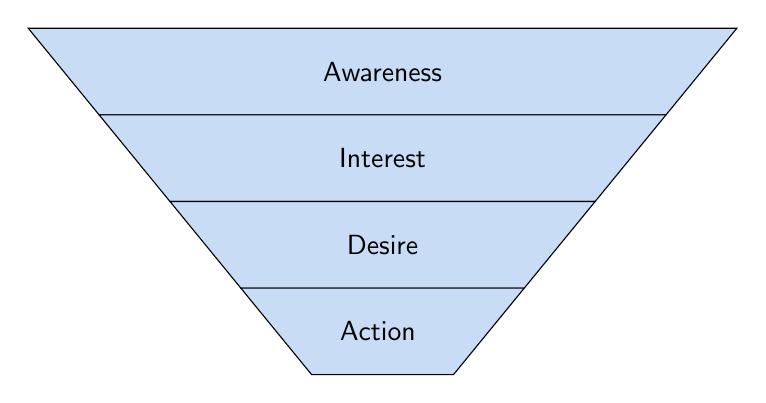
\begin{tikzpicture}[font=\sffamily, align=center]

        % Farben
        \definecolor{lightblue}{RGB}{200,220,245}

        % Trichter (invers)
        \def\levels{
            {Awareness},
            {Interest},
            {Desire},
            {Action}
        }
        % Maße
        \def\width{9}    % obere Breite
        \def\height{1.1} % Höhe jeder Ebene
        \def\num{4}      % Anzahl der Ebenen

        % Zeichne den invertierten Trichter
        \foreach \i [count=\n from 0] in \levels {
            \pgfmathsetmacro{\topwidth}{\width*(1 - (\n)/(\num+1))}
            \pgfmathsetmacro{\bottomwidth}{\width*(1 - (\n+1)/(\num+1))}
            \pgfmathsetmacro{\yshift}{-\n*\height}
            \draw[fill=lightblue, draw=black] 
                (-\topwidth/2, \yshift) -- (\topwidth/2, \yshift)
                -- (\bottomwidth/2, \yshift - \height) -- (-\bottomwidth/2, \yshift - \height)
                -- cycle;
            \node at (0, \yshift - 0.5*\height) {\i};
        }

    \end{tikzpicture}

    \caption{Sales Funnel \cite{Steuernagel2021, WengerLeadmanagement2021}}
    \label{fig:sales_funnel}
    
\end{figure}



\section{Lead Funnel}

\begin{figure}
    \centering
    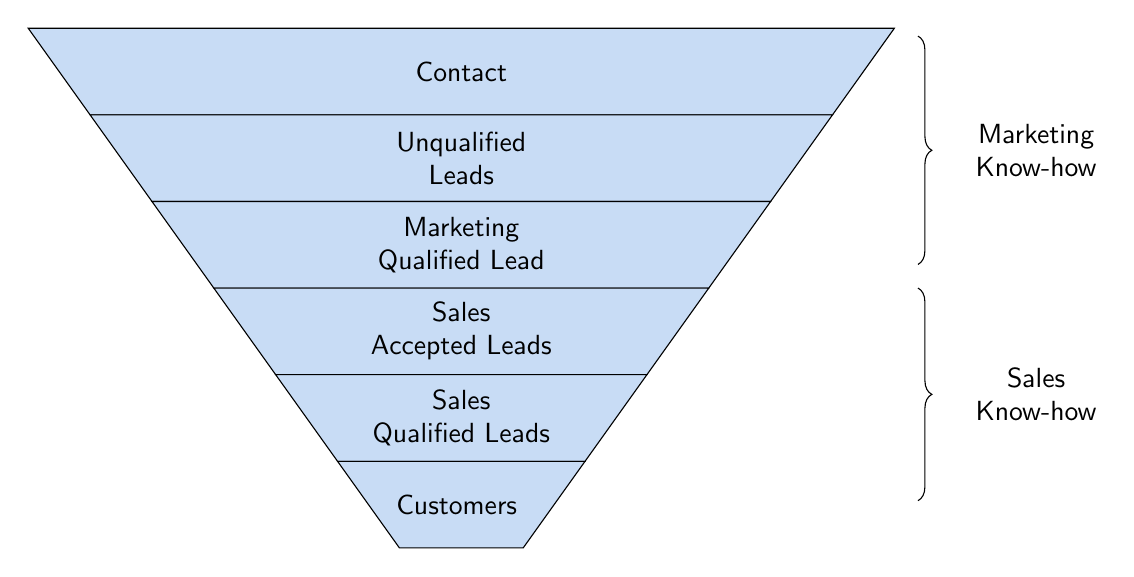
\begin{tikzpicture}[font=\sffamily, align=center]

        % Farben
        \definecolor{lightblue}{RGB}{200,220,245}

        % Trichter (invers)
        \def\levels{
            {Contact},
            {Unqualified\\Leads},
            {Marketing\\Qualified Lead},
            {Sales\\Accepted Leads},
            {Sales\\Qualified Leads},
            {Customers}
        }

        % Maße
        \def\width{11}    % obere Breite
        \def\height{1.1} % Höhe jeder Ebene
        \def\num{6}      % Anzahl der Ebenen

        % Zeichne den invertierten Trichter
        \foreach \i [count=\n from 0] in \levels {
            \pgfmathsetmacro{\topwidth}{\width*(1 - (\n)/(\num+1))}
            \pgfmathsetmacro{\bottomwidth}{\width*(1 - (\n+1)/(\num+1))}
            \pgfmathsetmacro{\yshift}{-\n*\height}
            \draw[fill=lightblue, draw=black] 
                (-\topwidth/2, \yshift) -- (\topwidth/2, \yshift)
                -- (\bottomwidth/2, \yshift - \height) -- (-\bottomwidth/2, \yshift - \height)
                -- cycle;
            \node at (0, \yshift - 0.5*\height) {\i};
        }

        % Klammern und Beschriftung rechts
        \draw [decorate, decoration={brace, amplitude=5pt}] 
            (5.8, -0.1) -- (5.8, -3.0) node[midway, xshift=1.5cm, align=center]{Marketing\\Know-how};

        \draw [decorate, decoration={brace, amplitude=5pt}] 
            (5.8, -3.3) -- (5.8, -6.0) node[midway, xshift=1.5cm, align=center]{Sales\\Know-how};

        
    \end{tikzpicture}

    \caption{Lead funnel \cite{WengerLeadmanagement2021}}
    \label{fig:lead_funnel}
\end{figure}

After the potential customer went through the \ac{aida} model and is ready to perform action (e.g. placing an offer, visiting a website, making a call), his journey continues with the Lead Funnel.
The first three steps are mostly managed by marketing departments and their success relies on Marketing Know-how (cf. figure \ref{fig:lead_funnel}) \cite{Steuernagel2021}. The first one of these is a phase called \textbf{Contact}. Here the potential customer gets in first contact with the company, e.g. though filling out a form on a website. 

Directly afterwards, the \textbf{Unqualified Lead} is created. The task of the marketing department is now to gather as much information as possible and decide whether the individual fits the general target profile. The goal of this phase is therefore to enrich the contact with basic demographic and company-related data that allows for an initial qualification \cite{Steuernagel2021, WengerLeadmanagement2021}.

Once these criteria are met, the prospect evolves into a \textbf{Marketing Qualified Lead}. While much of the early-stage qualification is driven by digital marketing automation, meaningful qualification increasingly requires human interaction as prospects move closer to a potential purchase \cite{Steuernagel2021}. Marketing typically decides whether the lead operates within the relevant target group that is supposed to be addressed. These insights are important information before a lead can be handed over to the sales department. 

If all criteria is met, the next stage, \textbf{Sales Accepted Lead}, marks the point where the sales team formally acknowledges the lead as relevant and takes the next actions. From that point on, the success relies on Sales Know-how \cite{WengerLeadmanagement2021}.

Historically, frameworks such as \ac{bant} were used to reach the \textbf{Sales Qualified Lead} state, whereas today more sophisticated methodologies like \ac{meddic} or \ac{champ} help sales teams evaluate opportunities in a structured and data-driven manner.

At the very end of the funnel, the prospect turns into a real \textbf{customer}. With that, the lead management process ends. Yet, the customer contact should not suddenly stop. Literature describes several customer retention programs to boost customer loyalty after the first initial sale \cite{Steuernagel2021}. However, they are not part of this project paper.


\section{Performance Metrics}
\label{sec:performance-metrics}

This section introduces the most important \ac{kpi}s inside Lead Management. In general, literature differentiates between metrics built for \textbf{lead scoring}, answering the question \textit{"how good is this lead?"} and \textbf{process performance metrics} designed for rating the lead management itself to answer the question \textit{"how good is the lead management?"} \cite{pedowitz2025kpis, Wu2024lead_scoring}.

In 2023, \citeauthor{Wu2024lead_scoring} performed a systematic literature review on the state of lead scoring metrics.
Their review spans 44 academic and industrial studies and identifies traditional scoring mechanisms but also modern data-driven predictive models. The authors highlight that predictive lead scoring approaches, such as decision trees and random forests, consistently outperform traditional techniques in terms of sales performance outcomes. Traditional techniques include \ac{kpi}s such as conversion rates, profitability, and cost efficiency \cite{Wu2024lead_scoring}. 

Among the process metrics, lead conversion rate emerges as the most frequently used performance measurement, followed by cost reduction, number of qualified leads and annual revenue \cite{Wu2024lead_scoring}. 

Some of \citeauthor{Wu2024lead_scoring}s mentioned \ac{kpi}s are presented in table \ref{sec:performance-metrics}. They will be used in chapter four to analyze the case study at Bosch.

\begin{table}
\centering
\renewcommand{\arraystretch}{1.3}

\begin{tabular}{p{2.5cm} | p{5.5cm} | >{$}c<{$}}

\textbf{Metric} & \textbf{Meaning} & \textbf{Formula} \\
\hline
Lead Cycle Time &
Time from lead creation until qualification or final closure. &
Date_{Closure} - Date_{Creation} \\
\hline
Time-to-First-Touch &
Time until first contact by Marketing or Sales after lead creation. &
Date_{FirstContact} - Date_{Creation} \\
\hline
Throughput Rate &
Number of leads processed in a defined time period. &
\frac{Total Leads Processed}{Time Period} \\
\hline
Conversion Rate &
Percentage of leads that move from one funnel stage to the next.
 &
\frac{Leads in Next Stage}{Leads in Current Stage} \times 100 \\
\hline
Lead Leakage Rate &
Proportion of leads dropping out between two stages. &
\frac{Leads Lost}{Leads Entering Stage} \times 100 \\
\hline
Sales Cycle Duration &
Average duration from SQL qualification to closed deal.
 &
Date_{Closure} - Date_{Qualification} \\
\hline
Cost per Lead &
Marketing and sales spend divided by the number of leads.
&
\frac{Total Marketing + Sales Cost}{Number of Leads} \\
\hline
Cost per Order &
Total cost per successfully closed sale.
 &
\frac{Total Marketing + Sales Cost}{Number of Closed Deals} \\
\end{tabular}

\caption{Lead Management Process KPIs \cite{pedowitz2025kpis, haufe2018vierkpis}}
\label{tab:lead_process_kpis}
\end{table}

In general, Lead Management is very rarely connected with Data Mining, not even speaking of Process Mining.  In one of \citeauthor{LeadmanagementDataMining2021} paper's called \textit{``Lead management optimization using data mining: A case in the telecommunications sector''} from 2021, they cite that only nine different papers existed on the relationship between lead management and data mining. In 2025, not much has changed in the perspective of Process Mining. A search for the string \textit{``process mining lead management''} even returns zero matching articles on Google Scholar. This indicates the research that still has to be performed on this topic \cite{LeadmanagementDataMining2021}.

%Umbruch vor dem Chapter Analysis
\addtocontents{toc}{\protect\newpage}
\chapter{Analysis}

This section aims to apply the knowledge gained from the previous sections to the example of Bosch. Bosch is a engineering and technology company founded by Robert Bosch in Stuttgart in 1886. The Bosch Group is divided into several business sectors, namely Mobility, Consumer Goods, Industrial Technology and Building Technology, adding up to a total revenue of 90,3 Billion euros in 2024. 
Bosch Home Comfort is part of the Industrial Technology and Building Technology sector, with a total revenue of 9 Billion euros \cite{bosch-facts-figures-2024}. On their website \url{https://www.bosch-homecomfort.com/de} end customers, businesses, and wholesalers can find multiple products on heating and well being, such as heat pumps, air conditioning, and condensing gas boilers. Especially end customers are offered with a button that allows them to ask for a tentative offer. After clicking, the user is required to fill out a form with some mandatory information (see figure \ref{fig:boschhomepage}) about their house, namely:

\begin{enumerate}
    \item Bewitched heating technology (e.g. heat pump or gas)
    \item Reason for interest (e.g. renovation)
    \item Building year (of house)
    \item Living area
    \item Energy consumption
    \item Bewitched installer in living area
    \item Bewitched starting date
    \item Number of inhabitants
    \item Kind of radiators (e.g. floor heating)
    \item Placement (of outdoor unit).
\end{enumerate}

After confirming and submitting the form, the lead is processed and stored within a relational database. 

Upon lead creation, three installers located in closest distance to the end customer’s residence are notified via both e-mail and SMS. Of these three, the two fastest respondents have the opportunity to accept the lead and submit an individual offer. The remaining installer receives a “Lead Missed” notification. Once the offers have been transmitted to the end customer, he may either accept or reject each proposal. If one of the offers is accepted, the lead is updated accordingly to final status ``sold''.

\begin{figure}
    \centering
    \includegraphics[width=\linewidth]{images/Bosch_Homepage_Lead.png}
    \caption{Bosch Lead Generation \cite{boschhomepage}}
    \label{fig:boschhomepage}
\end{figure}

As there are many different parties involved, this process has a great degree of variation. While they may share common milestones, such as \textit{LeadCreated}, \textit{LeadAccepted}, or \textit{LeadSold} the activities that occur between these stages can differ substantially depending on customer needs and the specific characteristics of the product or service involved \cite{Bernard2016SalesProcessMining}. As a result, sales processes rarely follow a strict and understandable trace and are considered spaghetti processes (compare section \ref{sec:lasagneshaphetti}). 

Instead, they adapt flexibly to the situational context. Moreover, sales processes can terminate at any point, as customers may switch to a competitor whenever they encounter a more attractive offer (cf. section \ref{sec:sales_funnel}) \cite{Vossebein2024LeadManagement}.

During analysis, this paper follows the \ac{llcm}. Therefore, the next sections will reflect the five different stages of that framework. Bosch Home Comfort has little experience in process mining. Since Bosch is currently performing the SAP S/4 roll-out in all of its operating countries, a pilot in Poland has been set up to start working with both Process Mining offered by Celonis in combination with the new \ac{erp} system. In the german market, there is no experience on process mining so far. 
As \citeauthor{AalstSpaghetti} recommends companies without much process mining experience to follow a question-driven approach, this chapter aims to answer the questions that were set up during a kick off meeting at the start of this project. Instead of starting with data exploration or pre-selected process KPIs, the method encourages analysts to begin with the problems and uncertainties raised by involved parties \cite{AalstSpaghetti}.

\section{Planning}
\label{sec:question}

During the initial kick-off meeting, Sales, Marketing and IT (called \ac{bdo}) defined several questions that should be answered through Process Mining. These questions reflect the information needs and uncertainties of the departments which could not be answered through Data Mining and an existing PowerBI Dashboard. To create some structure, the questions are put inside four different categories, accordingly to the phase of the Lead Management process: 

\newpage
\textbf{Lead Creation}
\begin{enumerate}
    \item Is there a specific lead path, which most of the users go through while creating a lead?
    \item Do users stay very long at one question as they do not know what to answer?
    \item Is there a specific lead path, in which users start and in which most users exit the \ac{lmt}?
\end{enumerate}

\textbf{Lead Matching}
\begin{enumerate}
    \item Is there a coincidence overall from rejected/missed leads? Regarding
    \begin{enumerate}
        \item Lead source
        \item Technology
        \item Lead use case
        \item Area
    \end{enumerate}
    \item How long does it take overall until a lead is accepted? 
    \item How long does it take per technology until a lead is accepted? 
\end{enumerate}

\textbf{Lead In Progress}
\begin{enumerate}
    \item How long does it take until a lead is set in progress?
    \item Are there leads which are never set in progress? And if so, why?
\end{enumerate}
\textbf{Lead Completion}
\begin{enumerate}
    \item Which kind of leads are mostly sold / not sold overall?
    \item Which kind of leads are mostly sold / not sold from a specific installer?
    \item Which installers have the highest probability to get the lead done if it was forwarded after not matchable?


\end{enumerate}

\newpage

\section{Extraction}

All data extraction and engineering is done via a Datalake Cloud Software called ``Databricks''. Databricks describes itself as
\begin{quote}
    \textit{``a unified, open analytics platform for building, deploying, sharing, and maintaining enterprise-grade data, analytics, and AI solutions at scale.'' }\cite{databricks_intro_2025}
\end{quote}

It is offered on both Cloud Computing Softwares \ac{aws} and Microsoft Azure. Originally, Databricks started as a runtime for PySpark Notebooks and evolved into a platform that supports multiple file formats and serves as central data hub for businesses. A typical component of Databricks is the so-called ``Unity Catalog'' in which data is stored in tables that exist of multiple parquet files \cite{databricks_intro_2025}. This allows a version control and fictional data quality levels (often called \textit{\mbox{Bronze-,}} \textit{Silver-} and \textit{Gold}-Layer). The data quality rises from bronze to gold, forming a pipeline shown in figure \ref{fig:databricks_architechture}. Databricks itself calls this principal ``Medallion Architecture''  \cite{DatabricksMedallionArchitecture}. This feature is also used inside this project paper work, since the lead management data is stored in two sources, the website (see figure \ref{fig:boschhomepage}) data that is stored via Google Analytics 4 inside a Google Big Query database and second the matching tool from Bosch that stores its data inside an Azure \ac{sql} database. Both can be connected via a Session and User ID that are transferred after the lead is submitted on the website.

\begin{figure}
    \centering
    \includegraphics[width=\linewidth]{images/Databricks_Modelling.png}
    \caption{Databricks Datalake Architecture \cite{DatabricksMedallionArchitecture}}
    \label{fig:databricks_architechture}
\end{figure}

\subsection{Feature Selection}

As mentioned by Aalst, a minimum event log consists of a case ID, timestamp and event (see table \ref{tab:minimal_event_log}). Further attributes, such as users, groups, product data can be added to enhance filtering. In our example, the data is stored inside multiple tables inside a snowflake schema in Databricks. Therefore it is necessary to join, filter and extract the data in a way that it can be read by process intelligence tools. Celonis offers \ac{odbc}, meaning the software can be connected to one of the Databricks Warehouses and read the data in real time. Beneficial is the fact that all of the heavy data transformation is handled inside the Data Lake and Unity Catalog of Databricks. Therefore none of the data transformation needs to be done inside Celonis. A complete overview of all features that have been loaded and selected can be seen in tables \ref{tab:ga4_clickstream} and \ref{tab:features}.  

Additionally, the event and session data of Google Analytics is also stored inside a Big-Query Database. Since Google Analytics tracks a lot of data and not everything is necessary, the dataset is dropped to ten columns that were most useful during analysis.

\begin{table}[h!]
\centering
\begin{tabular}{l|l|p{7cm}}

\textbf{Column Name} & \textbf{Data Type} & \textbf{Meaning} \\
\hline
Lead\_ID & INTEGER & Unique identifier of the lead (primary key from the Lead table). \\
\hline
uuid\_user & STRING & Unique user identifier from GA4 user properties (\textit{uuid\_user}). Used to connect events to individual users. \\
\hline
ga\_session\_number & INTEGER & Sequential session number from GA4 (\textit{ga\_session\_number}), indicating which browsing session the event belongs to. \\
\hline
EventDate & TIMESTAMP & Event timestamp converted into ISO 8601 format (\textit{yyyy-MM-dd'T'HH:mm:ss.SSSXXX}). \\
\hline
event\_timestamp & BIGINT & Raw event timestamp in microseconds since Unix epoch. \\
\hline
event\_name & STRING & Name of the GA4 event, representing the user action type (e.g. \textit{lmt\_toolstart}). \\
\hline
event\_action & STRING & Action parameter of the event (e.g., \textit{click}, \textit{start}, \textit{submit}). Extracted from \textit{event\_params}. \\
\hline
event\_category & STRING & Category describing the group of the event (e.g., "Tool", "Navigation"). \\
\hline
event\_label & STRING & Label providing additional context, such as the name of the clicked element or tool.  \\
\hline
click\_order & INTEGER & Sequential index of the user’s click or interaction, calculated via \textit{ROW\_NUMBER()} based on timestamp order. \\

\end{tabular}
\caption{Description of columns returned by the GA4 \ac{sql} query}
\label{tab:ga4_clickstream}
\end{table}

Every trace can be distinguished by a case ID named ``Lead\_ID''. Together with a timestamp in column ``EventDate'' and the event in column ``Event'' this is enough data to perform process mining (compare table \ref{tab:minimal_event_log}). In total, ten different attributes have been added to the dataset to allow filtering based on different criteria. Some of these attributes relate to lead characteristics, such as requested technology (e.g. heat pump, air conditioning, gas or oil) or ``Usprung'', meaning ``Brand'' leads whose origin is the Bosch Homepage, as well as ``Installer'' leads whose origin are individual installer websites. Further attributes are associated with the installers receiving a lead, including their ``PartnerLevel'' (a fictional classification based on annual revenue) and ``KUNNR'', which represents the installer’s customer number within the \ac{erp} system.


\begin{table}[h!]
\centering
\begin{tabular}{l|l|p{7cm}}

\textbf{Column Name} & \textbf{Data Type} & \textbf{Meaning} \\
\hline
Lead\_ID & INTEGER  & Unique identifier of the lead (primary key from the Lead table). \\
\hline
Status &  STRING & Name of the current status of the lead (e.g., \textit{New}, \textit{Accepted}, \textit{InProgress}). \\
\hline
Marke & STRING & Brand or product line associated with the lead. \\
\hline
Ursprung &  STRING & Source of the lead. Can be either \textit{Installer} or \textit{Brand}.\\
\hline
CreatedAt & TIMESTAMP  & Date and time when the lead record was created. \\
\hline
PostalCode & STRING  & Postal code of the lead’s end customer address. \\
\hline
Hist\_ID & INTEGER  & Unique identifier for the installer that accepted the lead. \\
\hline
EventDate & TIMESTAMP  & Date and time when the history event occurred. \\
\hline
Event & STRING & Type of history event (e.g., status changed, lead updated). \\
\hline
KUNNR & VARCHAR  & Identifier for the installer that accepted the lead \\
\hline
PartnerLevel & STRING & Label describing the partner’s level or tier (e.g. Gold, Silver, Platinum). \\
\hline
VBH\_ID &  STRING & Sales representative ID connected to the installer. \\
\hline
Requested\_Tech & STRING & Requested technology of end customer (e.g. "heat pump"). \\

\end{tabular}
\caption{Description of columns returned by the \ac{lmt} \ac{sql} query}
\label{tab:features}
\end{table}

\newpage
\subsection{Pipeline}
After the features are selected and the dataset is designed, two tables were created inside the Gold-Layer of Databricks. One table is called ``celonis\_hat'', representing the Wizard data from Google Analytics. The other table is called ``celonis\_lmt'', containing the data from the Bosch-internal Lead Management tool.

\newpage
A scheduled job runs daily at 6 a.m. UTC to execute the SQL code shown in chapters \ref{sec:code_google_analytics} and \ref{sec:code_bosch_lmt} inside a Jupyter Notebook to overwrite the tables with new data. Celonis supports \ac{odbc} and can directly access the data stored inside Databricks. The two tables are combined inside Celonis Studio and an additional column called ``Source'' is added to allow filtering for only one of the two datasets (if this is necessary). Since the attribute columns are different, some analysis can only be done with a subset of the data, as the other half contains null values.
\clearpage
\section{Create Control-Flow Model}

Before creating the Control-Flow model, some general analysis of the dataset is performed to receive a better understanding of the event log. In total, the dataset consists of $2.877.657$ rows, whereby $1.731.188$ originate from the Google Analytics dataset and the other $1.146.469$ from the Bosch Lead Management Tool. The data reaches back until the 1$^{st}$ of January 2024. 
Number of leads created per day and click rates on the Bosch website are very seasonal. Especially during summer months in 2024 and 2025 a marketing campaign called ``Cool \#LikeABosch'' created a lot of traffic and interest in Bosch air conditioning products. On average, $46.87$ leads are created per calender day in the selected time frame. The distinct count of Leads created per day can be seen in figure \ref{fig:count_lead_ids}. 

To get a general overview of the dataset, a separate Celonis asset called \textit{View} was created to track measures. Inside \textit{Views}, visuals can be placed via Drag \& Drop and adjusted in size, color and description. The landing page of one \textit{View} is shown in figure \ref{fig:celonis_landing_page}. It contains general statistics such as \textit{Leads per Status}, \textit{Average Time to Complete per Partnerlevel} and \textit{Number of Leads per Technology} to gain a first overview. Slicers at the top allow page-specific filtering but Celonis also allows view-wide filtering inside the menu bar. Further \ac{kpi} Analysis will be performed 
later on.

\begin{figure}
    \centering
    \includegraphics[width=1.0\linewidth]{images/Screenshot_Leadcount.png}
    \caption{Distinct Count of Leads per CreateDate}
    \label{fig:count_lead_ids}
\end{figure}



Defining an integrated process model for both the Google Analytics Wizard data as well as the Lead Management Tool is a tough task. In Celonis Studio, this can be done with a tool called \ac{pam}. The \ac{pam} allows user to mine, model and perform conformance checking. It also allows a \ac{bpmn} diagram to be uploaded and analyzed afterwards with the data inside the knowledge model \cite{celonis_pam}.

Since the data set can be roughly distributed into two parts, namely the Wizard data from Google Analytics and the data from the Lead Management tool,  separate analysis is performed and the two charts are be connected afterwards in SAP Signavio.

\begin{figure}
    \centering
    \includegraphics[width=1.0\linewidth]{images/Celonis_View_Landing_Page.png}
    \caption{Celonis Landing Page}
    \label{fig:celonis_landing_page}
\end{figure}

\subsection{Wizard Data}

Traces within the Wizard dataset may vary depending on two distinct parameters:

\begin{enumerate}
    \item \textbf{Source URL}. Depending on the original URL, e.g. sub-page ``products'' or ``use cases'' (for reference, see \url{https://www.bosch-homecomfort.com/de/de/ocs/wohngebaeude/waermepumpen}). For example, if the end user views the heat pump subsection and clicks on lead management, the question which technology he would like to have is no longer displayed.
    \item \textbf{Selected Technology}. Depending on the bewitched product, some questions are only shown whether they are relevant for that very technology. For example, the event \textit{Answer\_AirConditionedRoom} is only relevant for the technology air conditioning.
\end{enumerate}
\newpage

\begin{figure}[h!]
    \centering
    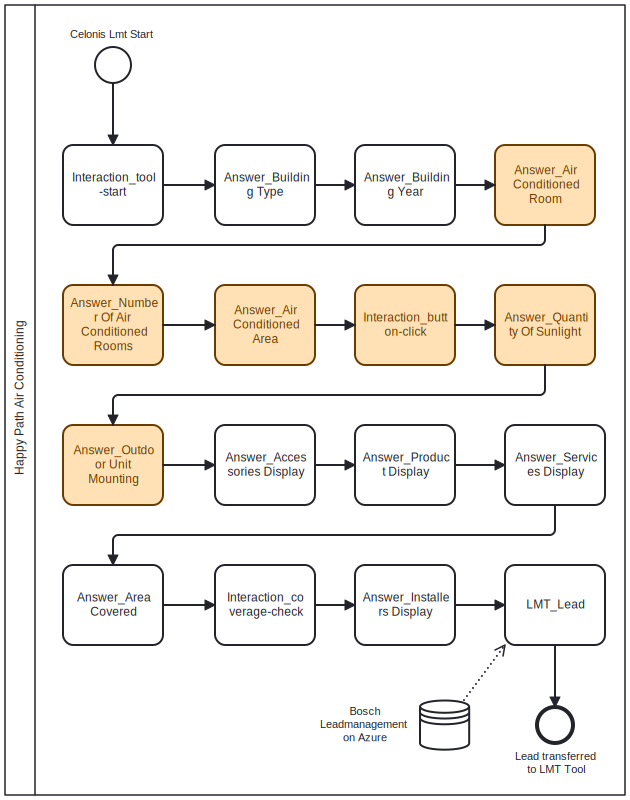
\includegraphics[width=0.8\linewidth]{images/bpmn/Wizard_Happy_Path_AirConditioning_Pool.pdf}
    \caption{Happy Path of Wizard data}
    \label{fig_happy_path_wizard}
\end{figure}


Figure \ref{fig_happy_path_wizard} shows the ``happy path'', meaning the most frequent trace of Wizard Data of the german Bosch homepage. As most leads were created for air conditioning technology, this trace represents a air conditioning flow. Therefore, there are some specific questions (e.g. area of placement of outdoor unit) to AC, which are highlighted yellow. 
Particularly noteworthy is that the first event is not \textit{Answer\_DesiredProduct}. This indicates that most leads did \textbf{not} originate from the general landing page but were instead initiated via product-specific sub-pages, such as those linked from social-media campaigns or similar channels.

\newpage
A complete process model of every possible technology selection can be seen inside the appendix in figure \ref{fig:wizard_flow_all_paths}. This model represents the ten most frequent variants, as well as specifically the trace for hybrid solutions (as they are selected very rarely and are not even part of the ten most frequent variants). It becomes clear that air conditioning traces differ a lot from traditional heating-only variants. E.g. the hybrid flow only differs in two question from a traditional ``heat pump'' flow, namely the events \textit{Answer\_Add\_Or\_New\_Hybrid} and \textit{Answer\_EnergySource\_Choices\_Hybrid}. The process chart in figure \ref{fig:wizard_flow_all_paths} covers \textbf{83\%} of all variants, meeting the requirements of \citeauthor{AalstSpaghetti} in chapter \ref{sec:lasagneshaphetti}.

A limitation from the Google Analytics dataset becomes visible in figure \ref{fig:wrong_modeling_wizard}. Sometimes, the next question shown inside the Wizard depends on the answer that was given in the previous question. However, this cannot be modeled by the heuristic miner inside Celonis. Either manual changes to the model have to be made or the selected answer must also be part of the event. Therefore, one could e.g. combine question and answer to distinguish between the traces of different selected models.

\begin{figure}
    \centering
    \includegraphics[width=0.9\linewidth]{images/bpmn/Incorrect_Modelling_Wizard.pdf}
    \caption{Wrong Modeling by Heuristic Miner}
    \label{fig:wrong_modeling_wizard}
\end{figure}

\newpage
\subsection{Lead Management Data}


As the dataset from the Lead Management Tool is way more complex, the control flow model is also looking more complex than the one from the Wizard data. In total, Celonis' Variant Explorer shows more than $2.000$ different variants of execution inside the log. For example, figure \ref{fig:lmt_modeling_5_frequent_variants} shows the control flow model with the five most frequent variants, figure \ref{fig:lmt_modeling_8_frequent_variants}  with the eight most frequent variants in comparison, growing rapidly in size. This model covers only \textbf{$31\%$} of all traces, therefore we can say that it does not meet the quality criteria of Section 2. Even by modeling only one installer (namely the one who sold the lead) instead of all potential three, no fitness above $80\%$ was achieved. While including additional variants marginally improves fitness, it also leads to a much larger increase in model complexity. Following the principle of Occam’s razor (see figure \ref{fig:four_quality_dimensions}), further expansion of the control-flow model is not beneficial and therefore stopped.


A combined version of both the Wizard data as well as the \ac{lmt} data with the eight most frequent variants can be seen in figure \ref{fig:wizard_lmt_combined} inside the appendix. High resolution source files are available inside a GitHub Repository, see chapter \ref{github} for further information.

\begin{figure}
    \centering
    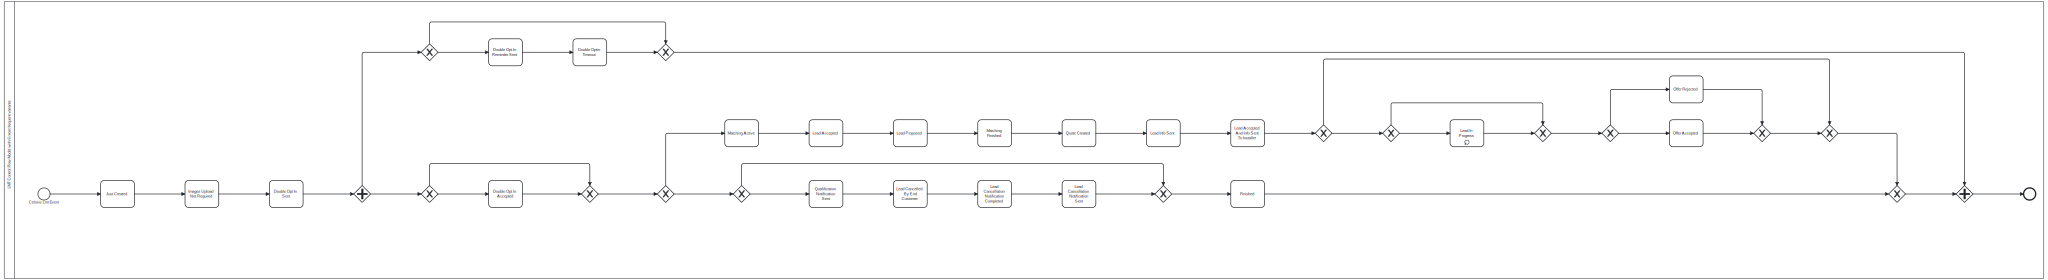
\includegraphics[width=1.0\linewidth]{images/bpmn/LMT_5_Variants.pdf}
    \caption{LMT Control Flow Model with 5 most frequent variants}
    \label{fig:lmt_modeling_5_frequent_variants}
\end{figure}

\begin{figure}
    \centering
    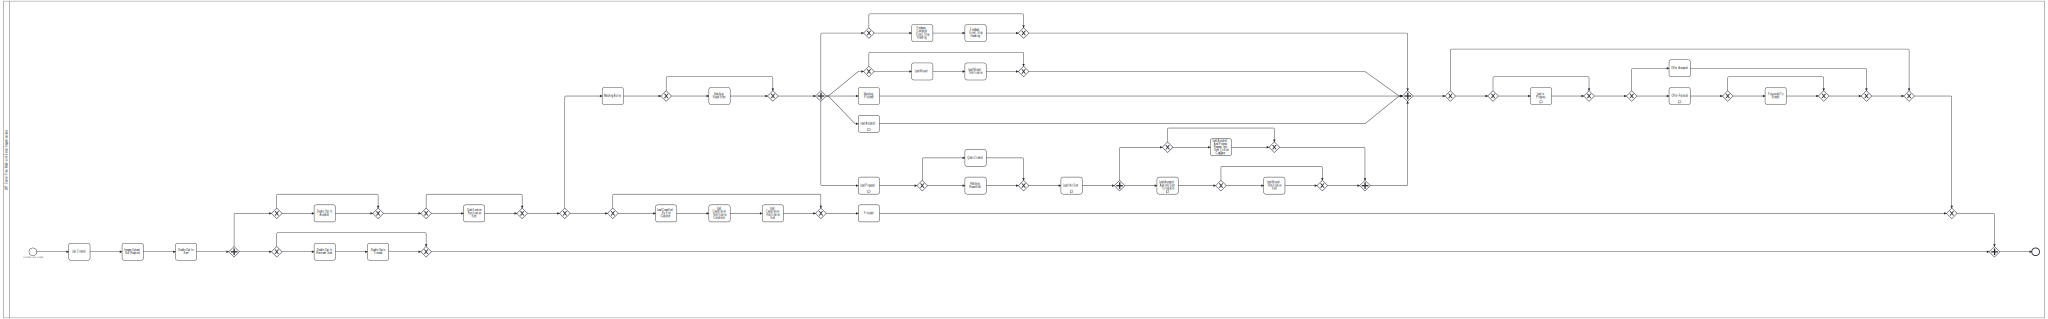
\includegraphics[width=1.0\linewidth]{images/bpmn/LMT_8_Variants.pdf}
    \caption{LMT Control Flow Model with 8 most frequent variants}
    \label{fig:lmt_modeling_8_frequent_variants}
\end{figure}


\clearpage
\section{Create Integrated Process Model}

These issues can be addressed during the creation of the integrated process model. In this step, \citeauthor{AalstSpaghetti} recommends refining the model not only structurally but also by incorporating organizational, temporal, and case-related information \cite{AalstSpaghetti}.

\textbf{Organizational Perspective} \\
One way of displaying the organizational perspective is the conversation model shown in figure \ref{fig:lmt_communication_diagram}. It shows the communication steps between different organizational units which are involved in the process, focusing on the exchange of information between the involved parties: \textit{Prospect}, \textit{Marketing Department}, \textit{Sales Department}, \textit{Installer}, and \textit{Customer}. This diagram highlights the sequence of communication events without describing the internal decision logic or the exact activity flow. It shows how a lead is initiated by the prospect, transferred to the marketing department for qualification, and subsequently forwarded to the sales department, which then engages with installers. Once an installer provides the product or service, the prospect transforms into a customer.

\begin{figure}
    \centering
    \includegraphics[width=1.0\linewidth]{images/bpmn/Lead Process Organizational View_cropped_cropped.pdf}
    \caption{Lead Management Conversation Model}
    \label{fig:lmt_communication_diagram}
\end{figure}

\newpage
\textbf{Time Perspective} \\
The duration of process execution is strongly influenced by chosen technology, involved installers and the end customer. External factors (such as governmental subsidies, which are beyond the control of Bosch) play a significant  role. Consequently, no explicit temporal perspective has been programmed into the current version of lead management at Bosch. The only time-related aspect considered is a lead timeout, which triggers if a lead is not accepted by any installer within 15 working days. Recommendations regarding the specification of lead timeouts and the integration of a more comprehensive temporal perspective are discussed in the conclusion of this work. 

\textbf{Case Perspective} 

The case perspective of the lead management process can be seen in figure \ref{fig:lmt_case_perspective}. The process begins when a prospect visits the website and initiates the lead wizard. Depending on the chosen technology, especially whether a heat pump is selected, the lead management tool triggers different qualification logic within the marketing department. Following the completion of the online questionnaire, the marketing-qualified lead is forwarded to sales, where installer selection is initiated. The process model further differentiates between cases in which prospects select installers themselves and cases in which the system automatically proposes the closest installers. As described in the text, up to three installers are notified simultaneously, and the two fastest respondents have the opportunity to accept the lead.

\begin{figure}[h!]
    \centering
    \includegraphics[width=1.0\linewidth]{images/bpmn/Process_Chart_cropped.pdf}
    \caption{Lead Management Case Perspective}
    \label{fig:lmt_case_perspective}
\end{figure}

\newpage
\section{Support}
This chapter focuses on using real-time data from running cases to detect deviations, predict future outcomes (e.g., remaining processing time), and recommend actions based on historical data. The results can be delivered directly to end users \cite{AalstSpaghetti}.

\subsection{Further Development}
Since the Lead Management Tool is constantly being changed and new features are added, the integrated process model needs to be updated frequently. Solution to this problem could be a \textbf{time filter} of attribute "createdAt". Since the current models are built on top of an event log reaching back to 1$^{st}$ of January 2024, it allows behavior that will not happen in new leads. For example, there is an event called \textit{DAAQualificationSent} that was removed in November 2024 and is not relevant in conformance checking of new leads. At max, it should only appear in old process models of 2024. 

\subsection{Alerting}
Celonis offers notification and alerting functions inside the \ac{pam}. This means, near to real time Celonis can check for deviations and contact colleagues. This could either be an option for developers to check for functional deviations, or for operational support (e.g. one lead stays too long in one specific status).

\subsection{Ownership}
As this proof of concept was build by german sales division, it cannot be maintained by a sales department since it exceeds their responsibilities. Therefore it will be passed on to \ac{bdo} who will roll out the Celonis Dashboard for every country that participates in Lead Management. \ac{bdo} will also ensure centralized governance, ongoing maintenance, and consistent data quality across regions. 


\chapter{Insights and Improvements}
This chapter is supposed to answer the questions that were made during chapter \ref{sec:question}. The following questions are either answered through Discovery, Variant Explorer or \ac{pql} formulas  made up as \ac{kpi} inside the knowledge model of Celonis.

\section{Lead Creation}

\textit{Q1. Is there a specific lead path, which most of the users go through while creating a lead?}

This question can be answered through the Celonis Variant Explorer. The happy path of the wizard data can be seen in figure \ref{fig_happy_path_wizard} which shows the trace of air conditioning leads, since they were requested the most by prospects. Second most frequent variant are leads for heat pumps, which are included in figure \ref{fig:wizard_flow_all_paths} as well as the technologies "hybrid", "gas" and "oil". As the sequence of questions can differ from the source URL and selected answers, the coverage of the nine most frequent variants acceptable with around $80\%$ (see table \ref{tab:variant-explorer}).

\begin{table}[h]
\centering
\begin{tabular}{l | l | l | l }
\textbf{Variant} & \textbf{Count} & \textbf{Coverage} & \textbf{Average TPT} \\
\hline
$\#1$ & $15{.}060$ & $24.6\%$ & $49 s$ \\
\hline
$\#2$ & $8{.}820$ & $14.4\%$ & $1 min$ \\
\hline
$\#3$ & $5{.}940$ & $12.3\%$ & $35 s$ \\
\hline
$\#4$ & $4{.}990$ & $10.3\%$ & $44 s$ \\
\hline
$\#5$ & $4{.}440$ & $6.2\%$ & $1 min$ \\
\hline
$\#6$ & $4{.}040$ & $4.1\%$ & $38 s$ \\
\hline
$\#7$ & $3{.}410$ & $4.1\%$ & $50 s$ \\
\hline
$\#8$ & $3{.}320$ & $2.0\%$ & $2 min$ \\
\hline
$\#9$ & $2{.}940$ & $2.0\%$ & $59 s$ \\
\hline
$Others$ & $13{.}240$ & $20.0\%$ & $54 s$ \\
\hline
\end{tabular}
\caption{Most frequent process variants}
\label{tab:variant-explorer}
\end{table}

\textit{Q2. Do user stay very long at one question as they do not know what to answer?}

This can be analyzed through the Celonis Process Explorer. Since prospects may temporarily leave the browser tab (e.g., to attend to other activities), throughput times vary substantially between the mean and the median.
This difference is particularly shown for the transition from the first to the second question, as the wizard tool is launched automatically when the URL is opened. Consequently, the recorded time between the events \textit{Answer\_BuildingType} and \textit{Answer\_LeadPurpose} is approximately one hour on average, while the median duration is only four seconds. For this reason, the median throughput time is considered more representative and is used for further analysis.

The longest median time is observed on the question \textit{Answer\_ServicesDisplay} with 31 seconds, followed by \textit{Answer\_OutdoorUnitMounting} with 25 seconds. This can likely be described by the fact that the event \textit{Answer\_ServicesDisplay} presents a large amount of textual information, which prospects must first read before selecting one or more desired services or explicitly choosing none. Some of the services can be seen in figure \ref{fig:services_wizard}.

\begin{figure}
    \centering
    \includegraphics[width=0.6\linewidth]{images/Wizard_longest_Median.png}
    \caption{Longest Median of Process Explorer}
    \label{fig:median_answer_services_Displayed}
\end{figure}

\begin{figure}[h]
    \centering
    \includegraphics[width=1.0\linewidth]{images/Wizard_Services.png}
    \caption{Selectable Services of event "Answer\_ServicesDisplay"}
    \label{fig:services_wizard}
\end{figure}

The comparatively long median duration for the event \textit{Answer\_OutdoorUnitMounting} is unexpected, as this question is intended for informational purposes only. Prospects can select from the options \textit{balcony}, \textit{façade}, \textit{top floor}, and \textit{other}. 

However, the final decision regarding the placement of the outdoor unit is ultimately made by the installer. Additionally, there is a very high drop of rate at that event of $19\%$. Therefore it is suggested to\textbf{ remove} that question from the HAT. 

\textit{Q3. Is there a specific lead path, in which users start and in which most users exit the Lead Management (LMT)?}

This question can be answered by a combination of questions \textit{Q1} and \textit{Q2} via the Process Explorer. Most prospects ($33\%$) start the Lead Manageent with the event \textit{Answer\_BuidlingType} which indicates that the lead originated from social media, since the events \textit{Answer\_LeadPurpose} and \textit{Answer\_Technology} do not appear. The second most frequent entry point ($30\%$) is the event \textit{Answer\_LeadPurpose}, representing prospects who clicked on a product-specific sub-page (e.g., heat pumps) and afterwards started the tool. The other $27\%$ of prospects come from the general landing page of Bosch Home Comfort Germany, as they just clicked on "Individual Offer".

Highest Drop-Off rates can be seen after events \textit{Answer\_OutdoorUnitMounting} with $19\%$ of all traces that lead through this event being terminated, followed by \textit{Answer\_Transfer} (e.g. floor or wall heating) with $13\%$. The third-highest drop-off rate occurs at the event \textit{Answer\_ProductDisplay}, with $7\%$. All remaining events show comparatively low drop-off rates below $4\%$.

As lead qualification is performed at a later stage by the marketing department anyways, each lead is valuable at this early point in the process. Consequently, it is recommended to \textbf{redesign} questions associated with high drop-off rates in order to reduce early LMT leaving and enable a higher number of leads to be generated at the beginning of the process.
\\
\newpage
\section{Lead Matching}

\textit{Q1. Is there a coincidence overall from rejected/missed leads? Regarding
\begin{enumerate}[a)]
        \item Lead source
        \item Technology
        \item Lead use case
        \item Area
    \end{enumerate}
}

Since the status and potential success of a lead is based on multiple factors (such as personal fit between installer and prospect, timing, use case etc.), coincidences are hard to find. However, Celonis Views allow page wide filters based on attributes of the event log. Since the initial event log (compare table \ref{tab:features}) has a column called \textit{Status}, anomaly detection was performed on Status Levels ``LeadRejected'' and ``LeadMissed''. There is no difference in rejected/missed leads in terms of their lead source. 
Per Technology, it is noticeable that AirConditioning contains more leads which where missed and rejected. This again can be explained due to peak weeks in summer, where a high amount of leads could not be handled by installers. While excluding these weeks, all technologies have roughly the same percentage of rejected ($30\%$) and missed ($10\%$) leads. 

On both Status, there is no noticeable difference in areal distribution inside Germany. Bosch distributes Germany into ten different regions with different sizes and revenue. As Bosch is a south-western based company, traditionally lead management works best in the Stuttgart-region where the brand is well-known and trusted. Therefore the most rejected and missed leads are from the sales region of southern-west Germany (called 927), followed by the second-biggest region around Frankfurt (called 909). 

\newpage
\textit{Q2. How long does it take overall that a lead is accepted?} 

This question can be answered either through a Celonis component called ``Throughput Time Explore'' or via a \ac{pql} formula with the following code that basically describes the \ac{kpi} ``Time-to-First-Touch'' which was already presented in section \ref{sec:performance-metrics}.
\begin{lstlisting}[language=SQL]
AVG(
  CALC_THROUGHPUT(
    FIRST_OCCURRENCE['DoubleOptInAccepted'] TO
    FIRST_OCCURRENCE['LeadAccepted'],
    REMAP_TIMESTAMPS(
      "celonis_lmt"."EVENTDATE",
      HOURS
    )
  )
)
\end{lstlisting}

As figure \ref{fig:avg_tpt_LeadAccepted} shows, the average varies between $0$ to $1488$ hours. The average time is $52,1h$, the median time is $32,1h$ until a lead is accepted by the first installer. This broad discrepancy can vary based on multiple reasons, such as that leads are not sent to installers during the weekend, resulting in longer throughput times and some unattractive leads, which go through multiple matching rounds until they are first accepted. As Celonis clusters the columns in $16h$-intervals, one can clearly see that most leads are accepted during the first $16$ hours after creation.

\begin{figure}[h!]
    \centering
    \includegraphics[width=0.75\linewidth]{images/KPI_throughput_toAccept_average.png}
    \caption{Average Throughput Time to Event "LeadAccepted"}
    \label{fig:avg_tpt_LeadAccepted}
\end{figure}

\textit{Q3. How long does it take per technology until a lead is accepted?}

\begin{figure}[h!]
    \centering
    \includegraphics[width=1.0\linewidth]{images/KPI_throughput_toAccept_average_Technology.png}
    \caption{Average Throughput Time to Event "LeadAccepted" per Technology}
    \label{fig:avg_tpt_LeadAccepted_tech}
\end{figure}

Figure \ref{fig:avg_tpt_LeadAccepted_tech} shows the same time frame as figure \ref{fig:avg_tpt_LeadAccepted}, but this time plotted by requested technology. Warm water ($12,14h$) and  gas heating ($15,77h$) leads are accepted way faster than e.g. heat pump leads ($46,05h$). This could be explained by the fact that they require way less planning and are overall cheaper and faster to install. Heat pumps take the longest time until they are accepted, with $46,05h$  from created time to accepted time. Striking are throughput times of air conditioning leads. After research, this is again due to the fact that there were peak lead creation numbers during high temperature summer weeks, where installers could not handle all the leads and were late on accepting new ones.

\clearpage
\section{Lead InProgress}

\textit{Q1. How long does it take until a lead is set in progress?} 

Similar to \textit{Q3} of section Lead Matching, the analysis was done both through the component ``Throughput Time Explore'' and via a \ac{pql} formula with the following code:
\begin{lstlisting}[language=SQL]
AVG(
  CALC_THROUGHPUT(
    FIRST_OCCURRENCE['LeadAccepted'] TO
    FIRST_OCCURRENCE['LeadInProgress'],
    REMAP_TIMESTAMPS(
      "celonis_lmt"."EVENTDATE",
      HOURS
    )
  )
)
\end{lstlisting}

Figure \ref{fig:avg_tpt_InProgress} shows the distribution of throughput times between the first occurrence of the event \textit{DoubleOptInAccepted} and the last occurrence of \textit{LeadInProgress}. The average throughput time amounts to approximately $904$ hours, while the median is significantly lower at around $575$ hours, indicating a strongly right-skewed distribution.
Most leads are set in progress within the first few hundred hours, as reflected by the high frequency in the lower time bins. However, a considerable number of cases exhibit very long waiting times, with a maximum of more than $6.000$ hours. These long-running cases heavily influence the average and point towards process inefficiencies or exceptional situations such as missing resources or backlog accumulation. 

\begin{figure}
    \centering
    \includegraphics[width=0.75\linewidth]{images/KPI_throughput_toInProgress_average.png}
    \caption{Average Throughput Time to Event "InProgress"}
    \label{fig:avg_tpt_InProgress}
\end{figure}

\textit{Q2. How long does it take per technology until is set in progress?}

\begin{figure}
    \centering
    \includegraphics[width=1.0\linewidth]{images/KPI_throughput_toInProgress_average_Technology.png}
    \caption{Average Throughput Time to Event "InProgress" per Technology}
    \label{fig:avg_tpt_InProgress_Tech}
\end{figure}

Figure \ref{fig:avg_tpt_InProgress_Tech} displays the average throughput time from event \textit{DoubleOptInAccepted} to event \textit{LeadInProgress}, broken down by requested technology. Clear differences between technologies can be observed.
Air conditioning leads reach the in-progress status fastest with an average of approximately $115$ hours, followed by heat pump and warm water leads. 

Gas heating and hybrid technologies show noticeably longer throughput times, while oil heating exhibits the highest average duration at roughly $186$ hours. These differences can largely be explained by varying planning complexity and installation requirements. Technologies such as air conditioning or warm water typically are cheaper and require less technical coordination. In contrast,  hybrid systems and heat pumps often involve more complex evaluations.
Overall, the figure underlines that technology choice is a key driver of throughput time.

\textit{Q3. Are there leads which are never set in progress? And if so, why?}

To answer that question, traces, where the event \textit{LeadInProgress} did not appear need to be filtered out. This can be done either via page-wide filters to analyze the \ac{kpi}s mentioned in chapter \ref{sec:performance-metrics} and figure \ref{fig:celonis_landing_page} or via the Celonis Process Explorer shown in figure \ref{fig:celonis_process_explorer}. The Process Explorer shows clearly, that $28\%$ of all $12.000$ leads in 2025 never run through the event \textit{LeadInProgress}, meaning they are accepted but never a product is offered by at least one installer. $17\%$ of all leads end at this event, meaning Bosch does not know, whether a product is sold or not. After excluding this event and plotting the leads by create date, there are spikes during summer, indicating that one reason is again the high air conditioning amount during high temperature summer weeks. However, it is more likely that a heat pump lead is never set \textit{InProgress} than a air conditioning lead, as heat pumps are over represented. Also, the sales region around Dortmund (called ``921'') is over represented. Further research has to be taken to answer that question more clearly.

\begin{figure}
    \centering
    \includegraphics[width=0.9\linewidth]{images/Process_Explorer_LeadInProgress.png}
    \caption{Celonis Process Explorer}
    \label{fig:celonis_process_explorer}
\end{figure}

\newpage
\section{Lead Completion}

\textit{Q1. Which kind of leads are mostly sold / not sold overall?}

This question can be answered using one of the metrics introduced in chapter \ref{sec:performance-metrics}. Namely, the sales rate can be calculated in \ac{pql} with this formula:

\begin{lstlisting}[language=SQL]
AVG(
  CASE(
    WHEN "celonis_lmt"."EVENTDATE" = 'Sold'
    THEN 1.0 ELSE 0.0
    END
   )
)
\end{lstlisting}

After creating this \ac{kpi}, a desired direction (in this case upwards) needs to be declared. Celonis offers a feature called ``Insight Explorer'' which makes suggestions and calculates the affect of that change to the \ac{kpi}.
Some suggestions are: 

\newpage
\begin{enumerate}
    \item Changing the question regarding energy consumption to a mandatory field can boost the sales rate (special type of \ac{kpi} ``Conversion Rate'' in table \ref{tab:lead_process_kpis}) from $16,58\%$ to $18,06\%$. This would roughly result in a revenue growth of $1.400.000$ \euro, assuming total lead volume stays the same and \ac{lmt} is accountable for $20\%$ of all sales.
    \item As lead purpose ``New Build'' has a $8,1\%$ lower sales rate than others, a differentiated prioritization strategy may be considered.
    \item Building types ``flat'' and semi detached flat have a much lower probability of being sold compared to other building types, mainly detached and semi detached (compare figure \ref{fig:celonis_insight_explorer}).
    \item Air conditioning, gas- and oil heating (all around $16\%$) have a much higher sales rate than heat pumps ($11,27\%$).
\end{enumerate}

\begin{figure}
    \centering
    \includegraphics[width=1.0\linewidth]{images/Celonis_Insight_Explorer.png}
    \caption{Example Suggestions of Insight Explorer}
    \label{fig:celonis_insight_explorer}
\end{figure}

\textit{Q2. Which kind of leads are mostly sold / not sold from a specific installer?}

To answer this question, all measures and visuals create from the question above are added a dimension from the event log attributes called ``KUNNR'', representing the customer number of every installer. Sales rate differs very much by installer, also the distribution of building types, purpose and requested technology. This makes clear that installers have preferences. However its not clear why metrics such as sales rate, conversion rate or time-to-first touch differ that much from installer to installer. 

One explanation might be that some installers take Lead Management more seriously, make better offers, or are more polite towards end customers, resulting in more sales.

\textit{Q3. Which installers have the highest probability to get the lead done if it was forwarded after not matchable?}

This question aims towards an event called \textit{ForwardedToInstaller} which only occurs after manual admin action. First, a lead has to be missed after the first two matching rounds. Afterwards, it reaches it final status \textit{NotMatchable} where the end customer is notified, that no suitable installer was found. If an admin interferes with that status, the lead is again ``open'' and can be sent to other installers. In 2025, this has happened $224$ times of around $19.643$ leads in total. Of these $224$ leads, only $2$ were confirmed sales. Because of this, the question cannot be answered, as the sample size is too small and therefore will be considered in future work.

\chapter{Conclusion}

This project set out to answer the research question: 
\begin{center}
    \textit{``How can process mining be utilized to optimize Lead Management and enhance sales performance at Robert Bosch GmbH?''} \\
\end{center}
Based on the conducted analysis of the Bosch Home Comfort Lead Management process, the results of chapters four and five show that Process Mining is a powerful and suitable approach to achieve both objectives.

By combining the two data sources Google Analytics wizard data and the internal Lead Management tool into a unified event log and analyzing it with Celonis, this study makes previously unknown process behavior transparent. The discovery phase reveals that Bosch’s Lead Management process matches the characteristics of a highly unorganized \textbf{spaghetti process}, as described by \citeauthor{AalstSpaghetti} in literature. Traditional reporting tools such as PowerBI are not able to capture this complexity, whereas Process Mining enables an view of actual process executions with building an integrated process model (\ref{fig:wizard_lmt_combined}) that reflects reality.

Regarding \textbf{Lead Management optimization}, Process Mining reveals multiple improvement opportunities within the process. First, the control-flow and variant analyses uncover typical and atypical lead paths, including a dominant ``happy path'' for air conditioning and numerous low-frequency variants that collectively account for more than half of all cases. Second, the throughput-time and drop-off analysis identifies critical points in wizard data, such as questions with unusually high median response times (requested services) and high drop-off rates. These findings lead to instant improvements, for example the removal of a question that causes early termination (question about placement of outdoor unit with $19\%$ drop-off).

Also, long waiting times between lead acceptance and the transition to status “in progress” for heat pump technology become visible. A significant share of leads never reaches the `ìn progress'' status at all.

 In terms of \textbf{enhancing sales performance}, the analysis showed how Process Mining can link process behavior to business outcomes. By combining lead attributes with \ac{kpi}s such as acceptance time and sales rate, the study identified patterns that otherwise would remain hidden. For instance, differences in acceptance time and conversion rates across technologies and installers highlight opportunities for differentiated lead routing and lead prioritization. Furthermore, the use of the Insight Explorer demonstrated how changes, such as making certain wizard fields mandatory or focusing on high-performing building types like ``detached flat'', can  improve sales-related \ac{kpi}s nearly $2\%$ and result in revenue growth (\ref{fig:celonis_insight_explorer}).

As this work focused on a proof of concept for the German market, the findings show high potential for a wider roll-out managed by a Bosch internal IT department (\ac{bdo}) in other countries that participate in Lead Management. 

\textbf{Critical Appraisal}

While this project papers shows the potential of Process Mining inside Lead Management, especially the \ac{llcm} showed limitations while creating the integrated process model. Since the Bosch-internal \ac{lmt} tool is under constant development and multiple parties (up to three different installers and end customers) are involved and can trigger processes at different times, there are more than $2.000$ different variants found by Celonis. Even with combining the $10$ most frequent versions, fitness remains low with $31\%$.

Also, results of this study should be interpreted with caution regarding generalization. The analysis focuses on the German market and a specific implementation of Bosch Home Comfort’s Lead Management process.
\addtocontents{lof}{\protect\newpage}
\appendix

\chapter{Process Models}
\label{github}


This section contains larger images of the process models compared to the versions inside the text. Alternatively, they are also uploaded to GitHub.

The GitHub Repository contains the diagrams in both their original source format and in high-resolution image format. It also includes the origiginal Latex-files to compile the final version of this project paper.

The repository is available to public at:

\noindent\url{https://github.com/wuestm/saps}



\begin{figure}[h]
    \centering
    \includegraphics[width=1.0\linewidth, angle=90, origin=c]{images/bpmn/Wizard_all_flows.pdf} 
    \caption{Wizard Data complete Control Flow Model}
    \label{fig:wizard_flow_all_paths}
\end{figure}

\begin{figure}
    \centering
    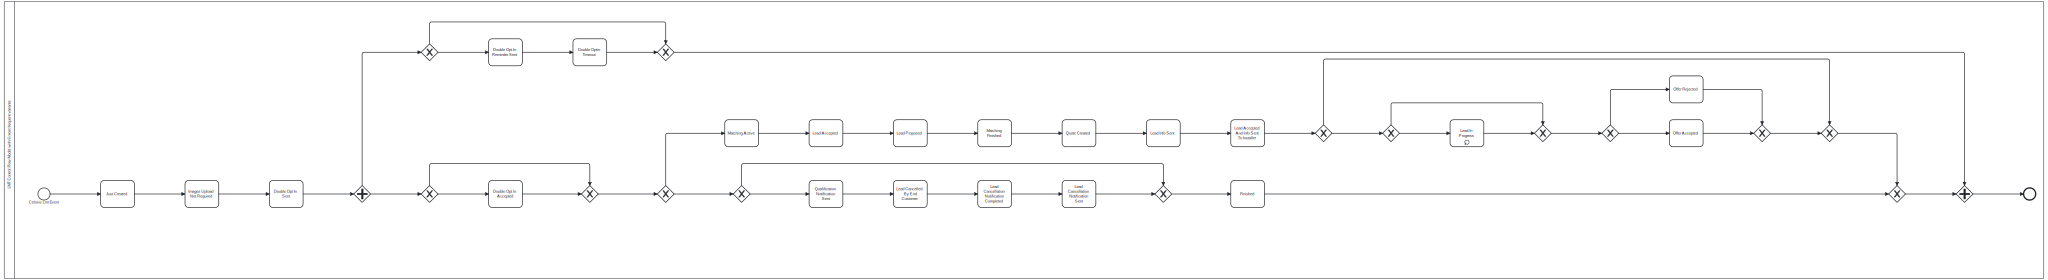
\includegraphics[width=1.0\linewidth, angle=90, origin=c]{images/bpmn/LMT_5_Variants.pdf}
    \caption{LMT Data Control Flow Model with 5 most frequent variants}
    \label{fig:appendix_LMT_5_variants}
\end{figure}

\begin{figure}
    \centering
    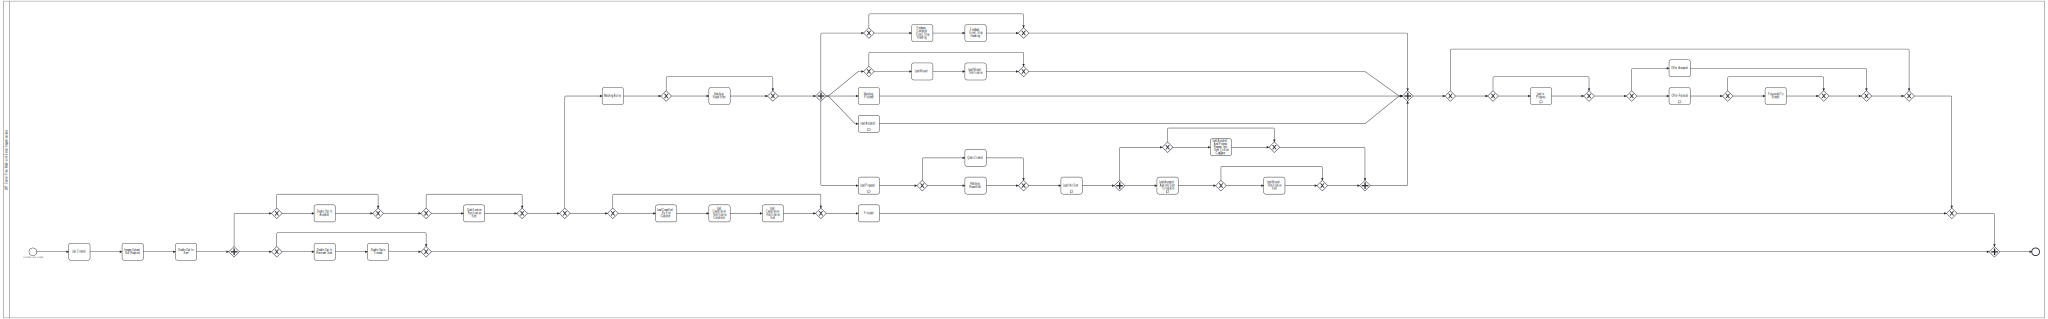
\includegraphics[width=1.0\linewidth, angle=90, origin=c]{images/bpmn/LMT_8_Variants.pdf}
    \caption{LMT Data Control Flow Model with 8 most frequent variants}
    \label{fig:appendix_LMT_5_variants}
\end{figure}

\begin{figure}
    \centering
    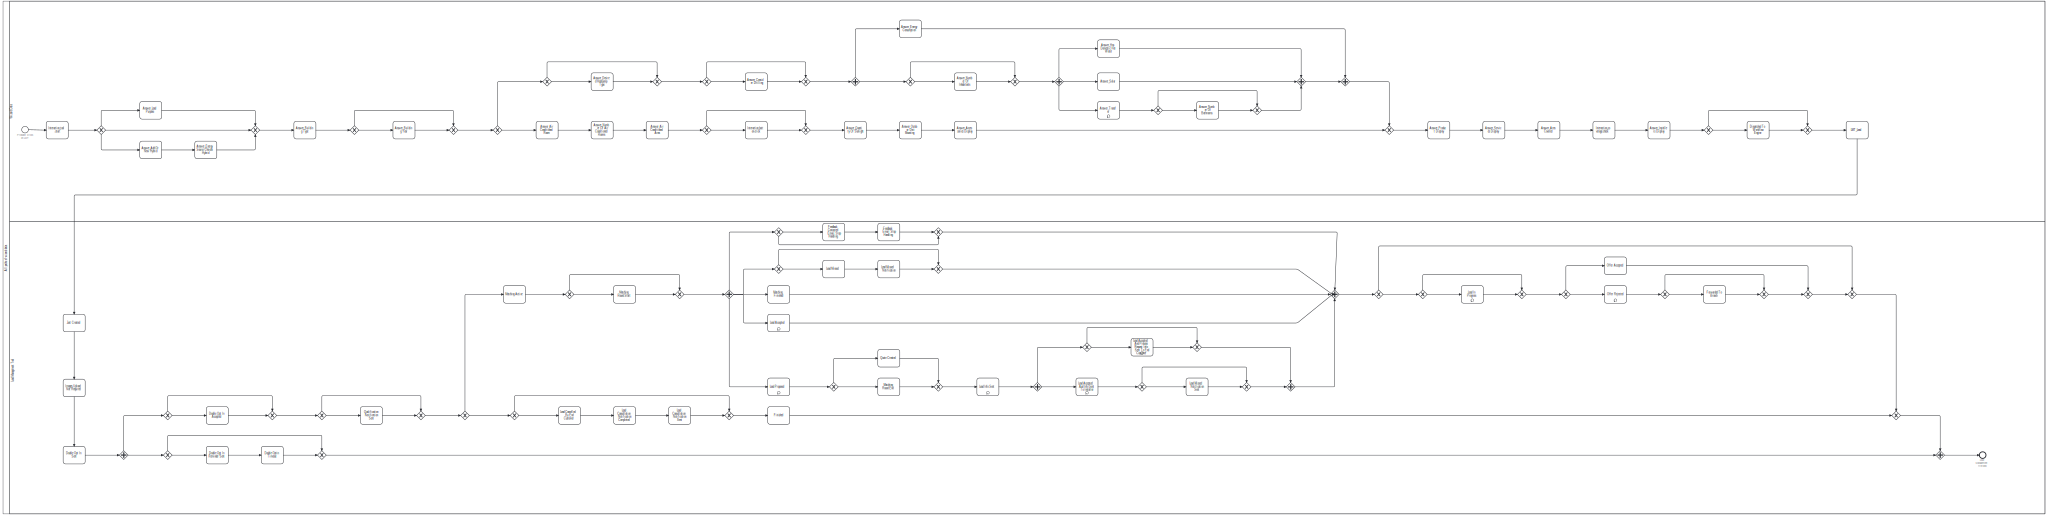
\includegraphics[width=1.3\linewidth, angle=90, origin=c]{images/bpmn/Wizard_LMT_combined_V2.pdf}
    \caption{Wizard and LMT combined Control Flow Model}
    \label{fig:wizard_lmt_combined}
\end{figure}
% hier Anhänge einbinden
\chapter{Source Code}

This chapter contains an abstract of source code used in this project paper.
\section{Google Analytics Extraction}
\label{sec:code_google_analytics}
\begin{lstlisting}[language=SQL, 
                    breaklines]
%sql


SELECT DISTINCT
  element_at(
    map_from_entries(
      transform(event_params, x -> (x.key, x.value.string_value))
    ),
    'event_label'
  ) AS event_label,
  element_at(
    map_from_entries(
      transform(event_params, x -> (x.key, CAST(x.value.int_value AS STRING)))
    ),
    'ga_session_number'
  ) AS ga_session_number
FROM hcdap_prod.bronze_ga4_website.ttmk_brandwebsite_bosch_de_de_326398072_ga4
WHERE event_name = 'lmt_toolstart'
  AND element_at(
        map_from_entries(
          transform(event_params, x -> (x.key, x.value.string_value))
        ),
        'event_label'
      ) IS NOT NULL;


-- Haupt-Query: Klickstrecke mit event_label + ga_session_number
SELECT
  lead.ID AS Lead_ID,
  uuid_user,
  ga_session_number,
  date_format(
    from_unixtime(event_timestamp / 1000000),
    "yyyy-MM-dd'T'HH:mm:ss.SSSXXX"
  ) AS EventDate,
  event_timestamp,
  event_name,
  event_action,
  event_category,
  event_label,
  ROW_NUMBER() OVER (PARTITION BY uuid_user ORDER BY event_timestamp ASC) AS click_order
FROM (
  SELECT
    event_timestamp,
    event_name,

    -- uuid_user aus user_properties
    element_at(
      map_from_entries(
        transform(user_properties, x -> (x.key, x.value.string_value))
      ),
      'uuid_user'
    ) AS uuid_user,

    -- ga_session_number aus event_params
    element_at(
      map_from_entries(
        transform(event_params, x -> (x.key, CAST(x.value.int_value AS STRING)))
      ),
      'ga_session_number'
    ) AS ga_session_number,

    -- event_action, category und label aus event_params
    element_at(
      map_from_entries(
        transform(event_params, x -> (x.key, x.value.string_value))
      ),
      'event_action'
    ) AS event_action,

    element_at(
      map_from_entries(
        transform(event_params, x -> (x.key, x.value.string_value))
      ),
      'event_category'
    ) AS event_category,

    element_at(
      map_from_entries(
        transform(event_params, x -> (x.key, x.value.string_value))
      ),
      'event_label'
    ) AS event_label

  FROM hcdap_prod.bronze_ga4_website.ttmk_brandwebsite_bosch_de_de_326398072_ga4
  WHERE event_name LIKE 'lmt_%'
) t

LEFT JOIN hcdap_prod.bronze_leadman.lead lead
  ON t.uuid_user = lead.UserUuid
WHERE uuid_user IS NOT NULL
--AND uuid_user = '8dc8f46e-6eab-4542-ae07-ffbf0d12bf01'
ORDER BY uuid_user ASC, click_order ASC;


\end{lstlisting}

\newpage
\section{Lead Extraction}
\label{sec:code_bosch_lmt}
\begin{lstlisting}[language=SQL, 
                    breaklines]
%sql
SELECT 
    lead.Id AS Lead_ID,
    lead.UserUuid AS uuid_user, 
    status.Name AS Status, 
    marke.Name AS Marke, 
    source.Name AS Ursprung,
    lead.CreatedAt,
    lead.PostalCode,
    lead.Latitude,
    lead.Longitude,
    hist.id AS Hist_ID,  
    hist.EventDate, 
    hist.Event, 
    installer.ParticipantId AS KUNNR,
    partnerlevels.Label AS PartnerLevel,
    Vbs.SalesRepId AS VBH_ID,
    CASE
    WHEN installer.ParticipantId IS NULL OR installer.ParticipantId = ''
        THEN 'General'
    WHEN MAX(CASE WHEN hist.Event = 'OfferAccepted' THEN 1 ELSE 0 END)
         OVER (PARTITION BY lead.Id, installer.ParticipantId) = 1
        THEN 'TRUE'
    ELSE 'FALSE'
    END AS Winning_INHB,
    get_json_object(lead.ExtraData, '$.QuestionAndAnswers.TechnologiesCategory') AS Requested_Tech, 
    get_json_object(lead.ExtraData, '$.QuestionAndAnswers.BuildingType') AS BuildingType,
    get_json_object(lead.ExtraData, '$.QuestionAndAnswers.BuildingYear') AS BuildingYear,
    get_json_object(lead.ExtraData, '$.QuestionAndAnswers.LeadPurpose') AS LeadPurpose,
    get_json_object(lead.ExtraData, '$.QuestionAndAnswers.DesiredHeatpumpType') AS DesiredHeatpumpType,
    get_json_object(lead.ExtraData, '$.QuestionAndAnswers.InstallationPlace') AS InstallationPlace,
    get_json_object(lead.ExtraData, '$.QuestionAndAnswers.HeatingArea') AS HeatingArea,
    get_json_object(lead.ExtraData, '$.QuestionAndAnswers.Transfer') AS Transfer,
    get_json_object(lead.Extradata, '$.QuestionAndAnswers.EnergyConsumption') AS EnergyConsumption,
    get_json_object(lead.Extradata, '$.QuestionAndAnswers.NumberOfInhabitants') AS NumberOfInhabitants,
    get_json_object(lead.Extradata, '$.QuestionAndAnswers.SelectedServices.Name') AS SelectedServicesName
-- '''  COUNT( *), lead.Id'''
    --lead.ExtraData
    
--* 
FROM hcdap_prod.bronze_leadman.lead lead
    LEFT JOIN hcdap_prod.bronze_leadman.brokerhistories hist
        ON lead.id = hist.LeadId
    LEFT JOIN hcdap_prod.bronze_leadman.leadconsumer leadconsu
        ON leadconsu.Id = hist.LeadConsumerId
    LEFT JOIN hcdap_prod.bronze_pp20.installermemberships installer 
        ON leadconsu.CompanyGuid = installer.Company_CompanyId
    LEFT JOIN hcdap_prod.bronze_pp20.installerpartnerlevels partnerlevels
        ON installer.PartnerLevel_Id = partnerlevels.Id
    LEFT JOIN hcdap_prod.bronze_pp20.installers installers 
        ON installer.Company_CompanyId = installers.CompanyId
    LEFT JOIN hcdap_prod.bronze_leadman.leadstatuslookup status 
        ON lead.Status = status.Id
    LEFT JOIN hcdap_prod.bronze_leadman.variant variante
        ON lead.VariantId = variante.Id
    LEFT JOIN hcdap_prod.bronze_leadman.leadsourcelookup source
        ON lead.Source = source.Id
    LEFT JOIN hcdap_prod.bronze_leadman.brandlookup marke
        ON variante.Brand = marke.Id
    LEFT JOIN hcdap_prod.bronze_leadman.wizard wizard 
        ON hist.LeadConsumerId = wizard.LeadConsumerId
    LEFT JOIN hcdap_prod.bronze_leadman.leadconsumerstatus leadstatus
        ON wizard.LeadConsumerId = leadstatus.LeadConsumerId
    LEFT JOIN hcdap_prod.bronze_pp20.salesreps VBs
        ON VBs.Id = installer.SalesRep_Id
    LEFT JOIN hcdap_prod.bronze_pp20.salesbranches Salesbranch
        ON Salesbranch.Id = VBs.SalesBranchId
    LEFT JOIN hcdap_prod.bronze_pp20.installertools tools
        ON tools.InstallerMembership_Id = installer.Id 
       AND tools.Tool = '1'  

WHERE 
    marke.Name = 'Bosch'
    AND lead.CreatedAt > '2024-01-01'
 --   AND lead.CreatedAt = '2025-08-11'
   -- AND LEFT(installer.ParticipantId, 2) = '39'
    AND variante.Country = "DE"
   -- AND lead.ID = '315498'


GROUP BY ALL 

\end{lstlisting}


\chapter{Declaration of Honor}  % Titel wie in der Vorlage

\parindent0pt
\parskip3ex

\def\dotsign{\xleaders\hbox to .2em{\d{}}\hfill\d{}}
\def\dashsign{\xleaders\hbox to .5em{\_}\hfill\_}

\textbf{Name:} \fullname \hfill \textbf{Student ID:} \matnr \vspace{2cm}

I hereby declare that I have written my Project Paper with the title

\begin{center}
    \textit{``\titel''}
\end{center}

independently and have not used any sources or aids other than those indicated. All literal quotations in the thesis have been clearly marked with quotation marks. The thesis has not been submitted in the same or a similar form for any other examination.  
The electronic version corresponds exactly to the printed version.  
The main text of the thesis comprises \textbf{10.915} words.

Stuttgart, 30.12.2025  % DATUM NOCH EINTRAGEN

\makebox[.5\linewidth][l]{Signature}\dotsign\smallskip\\
\hspace*{.5\linewidth} Moritz Wüst


\backmatter
\nocite{Knappen2009}
\nocite{Mittelbach2005}
\nocite{Schlosser2014}
\nocite{Sturm2012}
\nocite{Voss2010}

\printbibliography

\clearpage

\end{document}

